\chapter{Photon Reconstruction in \pandora}
\label{chap:Photon}

\chapterquote{Photons have mass? I didn��t even know they were Catholic.}%
{Woody Allen}

%\section{Introduction}

Photon reconstruction is an important part of \pandora reconstruction. A good photon reconstruction should provide a good single photon completeness and purity, as well as a good photon separation resolution. For many physics processes, heavy particles decaying into photons, such as \Ptau lepton and \Ppizero. Photon reconstruction is crucial for reconstructing these heavy particles.

The photon reconstruction presented in this chapter has improved the photon reconstruction completeness by reducing the fragments. The photon separation resolution has been improved as well. This work has been published in a conference proceeding \cite{Xu:2016rcz}. The improved   photon reconstruction has benefited many physics analyses involving photons in the final state. The most recent example is the  \HepProcess{\PHiggs \to \Pgamma \Pgamma} analysis at \rootS{3} at \CLIC \cite{Kacarevic:higgsToGammaGamma}.

%This set of photon related algorithms have been incorporated into the default reconstruction chain in \pandora. The \CLIC simulation studies have benefited from the improved photon reconstructions in various physics process, such as  \HepProcess{ \PHiggs \to \Pgamma \Pgamma}.

\begin{comment}
Since the discovery of a particle consistent with being the SM Higgs boson in LHC at 2012 \cite{Aad:2012tfa,Chatrchyan:2012ufa}, our understanding of Standard Model has improved greatly. Yet limited by the underlying QCD interaction from proton-anti-proton collision, one has great difficulty to measure the properties of the Higgs precisely. Next generation electron-positron linear collider could hopefully make precision measurements of the Higgs sector and the Top quark sector \cite{Abramowicz:2013tzc}.

The leading candidates for next generation electron-positron linear collider are the International Linear Collider (ILC) \cite{Brau:2007zza}, and the Compact Linear Collider (CLIC) \cite{Linssen:2012hp}. The ILC has developed two detector models, namely the International Large Detector (ILD) \cite{Abe:2010aa} and the Silicon Detector (SiD) \cite{Aihara:2010zz}. The CLIC has developed two slightly modified detector models based on ILD and SiD \cite{Linssen:2012hp}. One key common feature of these next generation electron-positron linear colliders is the high granular calorimeter, which provides a great spatial resolution at the cost of the energy resolution. Particle flow algorithms (PFA) benefit from the spatial resolution from calorimeters, together with tracking information, to provide excellent a jet energy resolution. PandoraPFA, the most complicated and the best performing one, provides a jet energy resolution of less than 3.5\%, which is required for W/Z separation \cite{Thomson:2009rp,Marshall:2013bda}.

\begin{figure}[tbph]
\centering
{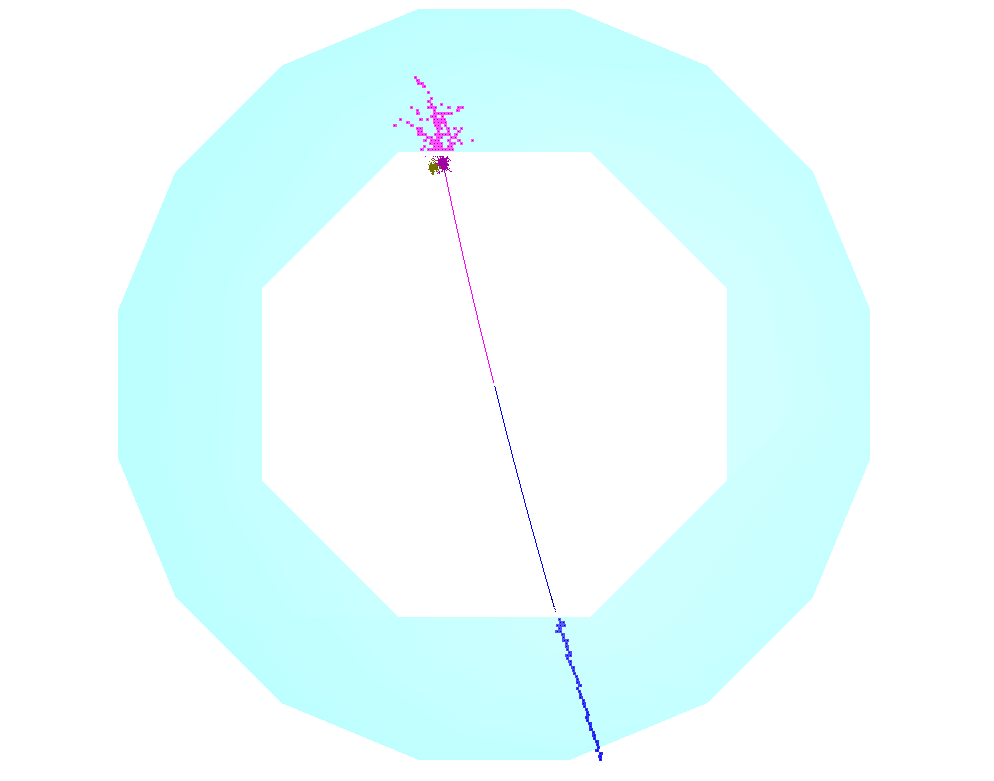
\includegraphics[width=0.5\textwidth]{images/tautauMod}}%

\caption{An event display of a simulated $\Pem\Pep\to \Ptauon\APtauon$ event. The blue region is the cross section of the Electromagnetic Calorimeter barrel region. The top $\Ptau$ decays into a charged $\Ppi$, two photons and neutrinos. The bottom $\Ptau$ decays into a muon and neutrinos.}
\label{fig:Tautau}
\end{figure}

Photon reconstruction is an important part of particle reconstruction. For many physics processes involving particles decaying into photons, such as $\Ptau$ lepton and $\Ppizero$, a good photon reconstruction, which provides a good single photon completeness and purity, as well as a good photon separation resolution, is crucial for reconstructing these particles.

\end{comment}
\section{Electromagnetic shower}

\section{Overview of photon reconstruction in PandoraPFA}

PandoraPFA provides a framework for particle reconstruction \cite{}, as described in \Chapter{chap:Reconstruction}. In the linear collider content, it has a vast library of algorithms developed through years by many people. Each algorithm addresses one topological issue in the particle reconstruction \cite{}. The essential part of the PandoraPFA is track-cluster association and reclustering to find the best track-cluster pair. Algorithms that removes trackless clusters, such as removing muon clusters or photon clusters, would provide a clean environment for the track-cluster association, hence improving the jet energy resolution.

Photon identification in the PandoraPFA has two main mechanisms. The basic mechanism (see \Section{sec:pandoraPFOcreation}) performs photon identification after track-cluster association and the reclustering processes. The second more sophisticated photon identification, the photon reconstruction algorithm, is performed before the track-cluster association and reclustering process. This algorithm identifies photon electromagnetic shower cores carefully in the dense jet environment.

The photon reconstruction algorithm in \pandora version 1 improves jet energy resolution by correctly identifying photon electromagnetic shower cores and leaving a cleaner environment for the track-cluster association. However, the peripheral calorimeter hits to the shower cores may be left as fragments, and reconstructed as separate particles. This lowers the reconstructed photon completeness and makes the number of reconstructed photons a less useful physical quantity. Also, the algorithm in \pandora version 1 leaves rooms for improvement of photon separation resolution.

This section presents a solution to the photon fragments issue. The newly introduced \pandora algorithms also improves the photon separation resolution. Algorithms related to photon reconstruction, fragmental removal and photon splitting, which are written or introduced by authors, will be discussed below.

%Three algorithm will be discussed: a rewritten sophisticated photon reconstruction algorithm, a photon fragment removal algorithm and a photons splitting algorithm.

%The testing simulated data in this paper are generated either by WHIZARD \cite{whizard} or by the simple HepEvt generator. Events are simulated with GEANT4 \cite{Agostinelli:2002hh} in MOKKA \cite{MoradeFreitas:2002kj}. Jet fragmentation was performed with PYTHIA \cite{Sjostrand:1995iq} and the particle reconstruction was done by PandoraPFA \cite{Marshall:2015rfa} in MARLIN reconstruction framework \cite{Gaede:2006pj}, in ILD\_o1\_v6 detector model. The iLCSoft v17-01-07 was used. Different versions of PandoraPFA were used for the comparison purpose.

\section{Photon reconstruction algorithm}
\label{sec:photonRecostrcution}
The photon reconstruction algorithm refers to the more sophisticated photon identification of the two main identification mechanisms, before the track-cluster association and reclustering process (see \Section{sec:particleID}). The algorithm has the following steps: coarsely forming photon clusters, reconstructing photon candidate, photon ID test, and optional fragment removals. Reconstructing photon candidate requires further explanation of the two dimensional peak finding algorithms in \Section{sec:peakFinding}. The photon ID test involves a multi dimensional likelihood classifier, which is described in \Section{sec:photonLikelihood}.

\subsection{Form photon clusters}

This step finds large potential photon clusters. All calorimeter hits in the \ECAL, which are not used in previous algorithms, are grouped into clusters using a cone based clustering algorithm.To find neutral photon clusters, which do not deposit energies in the tracking system, the cone clustering algorithm is seeded with energetic hits. The parameters for the cone clustering are generous, allowing potentially two or three photons in one cluster.

\subsection{Reconstruct photon candidates}
\label{sec:photonCandiate}

The large photon clusters are split into smaller photon candidates, using two-dimensional shower profiles. The candidates close to a track projection are deemed as non-photons. Identifying photon candidates within a large photon cluster relies on the characteristic electromagnetic showers, in particular the transverse distribution. A energetic photon or electron hits the absorber layers of the \ECAL, it initiates an electromagnetic shower, where electron pair production and bremsstrahlung produce more low-energy photons and electrons. The transverse distribution is characterised by a narrow cone, widening while the shower develops.

To view the transverse shower distribution, a two-dimensional energy deposition projection is constructed in the plane perpendicular to the direction of the cluster. \Figure{fig:photonPeakFinding} shows the energy deposition projection of two photons candidates. U and V axis are two arbitrary orthogonal axis in the transverse plane perpendicular to the direction of photons. Z axis shows the sum of the calorimeter hit energy in GeV. The bin size corresponds to the square \ECAL cell size.

\begin{figure}[tbph]
\centering
{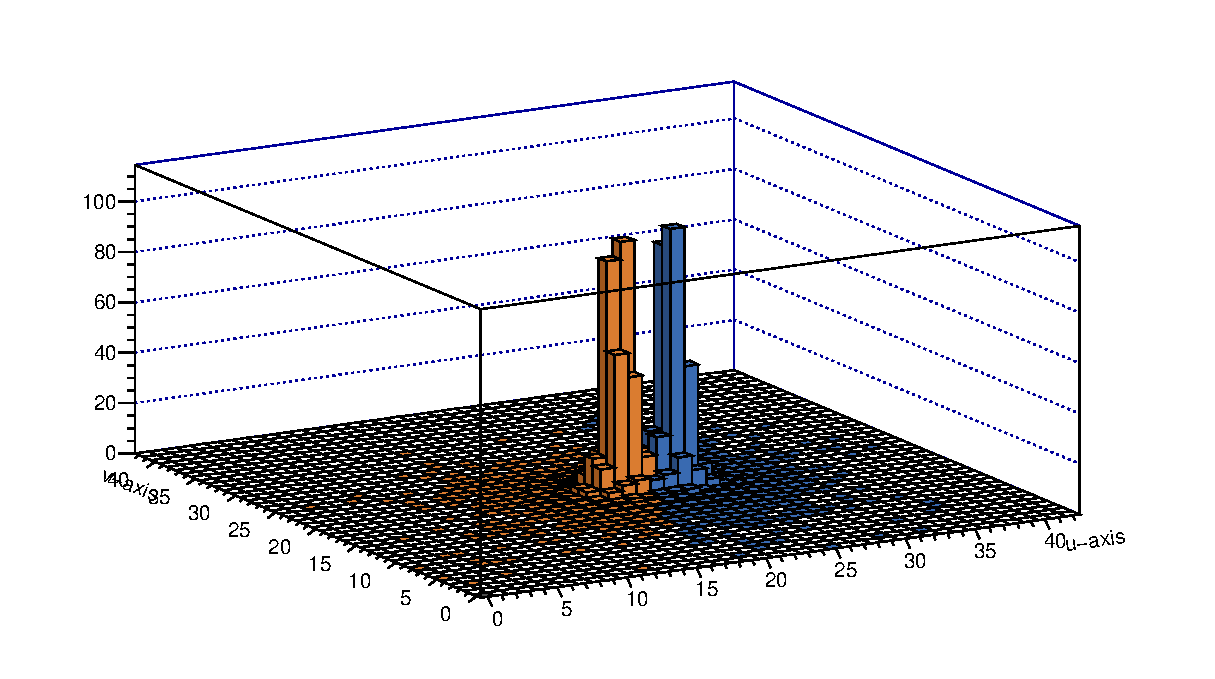
\includegraphics[width=0.5\textwidth]{photon/peakFinding}}%

\caption{Two 500\,GeV photons (yellow and blue), just resolved in the transverse plane perpendicular to the direction of the flight, of their energy deposition in electromagnetic calorimeter. U and V axis are two arbitrary axis perpendicular to each other in the plane. Z axis is the sum of the calorimeter hit energy in each particular bin in 2D plane in GeV.}
\label{fig:photonPeakFinding}
\end{figure}

By using the two-dimensional energy deposition projection, separating photons translates to separating peaks in the projection. Therefore a high performance two dimensional peak finding algorithm is the key to identify multiple photons. The peak finding algorithm will be discussed in \Section{sec:peakFinding}

The output of this step is a collection of photon candidates from a photon cluster, which will be fed to the photon ID test.

\subsection{Photon ID test}
\label{sec:photonIDtest}

Photon ID test decides if a a candidate is a photon. If a candidate is not a photon, the calorimeter hits of the candidate will be passed on to the next stage of the reconstruction.  The photon ID test is a multidimensional likelihood classifier. The classifier is trained with discriminating variables, which exploit features electromagnetic showers. The classifier will be discussed in \Section{}

\subsection{Photon Fragment removal}
\label{sec:photonRecoFragRemoval}
The optional photon fragment removal aims to merge small photon fragment to main photons. Since this step shares the same logic as the algorithm in \Section{}, only differing in the cut-off values for merging metrics, this step be discussed in \Section{}.

This step marks the end of the photon reconstruction algorithm. The output are a collection of reconstructed photons, separated from non-photon calorimeter hits.
%The candidate passed the test will be kept in a separate container for photons only

\section{Two dimensional peak finding algorithm for photon candidate}
\label{sec:peakFinding}

As discussed in \Section{sec:photonCandiate}, separating photon candidates from a cluster is same as identifying peaks in a two dimensional histogram. An example of two photons is shown in the \Figure{fig:photonPeakFinding}. The basic algorithm treats all clusters as potential photon clusters. Since charged hadrons would deposit tracks in the tracking system, extra care is taken when a cluster is close to the projection of the track in the front of the \ECAL. The basic peak finding algorithm has two main functions: identifying peaks, and assigning bins to peaks.

A two dimensional histogram is constructed using a plane orthogonal to the direction of the flight of the photon cluster. The U and V axis in \Figure{fig:photonPeakFinding} are two orthogonal axes in the plane. The width of the histogram is determined by the size of the \ECAL square cell. The calorimeter hits of the photon cluster are then projected onto the two dimensional histogram. The height of the bin is the sum of the calorimeter hit energies in the bin.

A local peak is defined as a bin where its height is above all eight neighbouring bins. After all peak bins are found, non-peak bins are associated to one peak bin, by choosing the peak bin that minimise the metric
\begin{equation}
\frac{d}{\sqrt{E_{peak}}}
\end{equation}
where $d$ is the Euclidean distance between a non-peak bin and a peak bin on the histrogram, and $E_{peak}$ is the height of the peak bin, which is the energy. Alternative metrics provided in the algorithm include $d$, $\frac{d}{{E_{peak}}}$, and $\frac{d}{{E_{peak}^2}}$. The default metric is chosen due to a good balance between distance and energy of the peak.

\subsection{Candidate close to track projection}

If a cluster or a photon candidate is close to the projection of the track in the front of the \ECAL, it is likely that the cluster or the candidate is a charged hadron. Misidentifying a charged hadron as a photon leads to significant degradation in reconstruction performance. However, if a photon next to a charged hadron is carefully reconstructed, the overall reconstruction is improved. Hence this step aims to carefully identifies photon candidate next to charged hadrons, by using track information and features of the electromagnetic shower. Photon induced electromagnetic shower in the \ECAL typically start in the first few layers. As the shower develops, the direction of the shower core does not change much.

If a peak bin is within the eight neighbouring bins of the track projection onto the two dimensional plane, the peak and its associated bins are flagged as non-photons. Furthermore, the \ECAL is sliced longitudinally to help identify photon candidates. For example, the default three slices will result in three \ECAL fiducial spaces, each contains space from the front of the \ECAL to a third, two thirds and the back of the \ECAL, respectively. The peaking finding algorithm is repeated for the same cluster divided in each \ECAL fiducial space. The peak is only preserved as a photon candidate if the peak exists in every fiducial space, and if its position is shifted by no more than one neighbouring bin between fiducial spaces.


\subsection{Peak filtering}

The performance of the two dimensional peaking finding algorithm is improved by clever programming and physics arguments. For a given two dimensional histogram, such as the one in \Figure{fig:photonPeakFinding}, major peaks most likely correspond to physical photons, while the minor peaks more likely come from fluctuations in energy deposition. To select major peaks, every time after non-peak bins are associated with peak bins, minor peaks with fewer than three bins associated (including the peak bin) are discarded. These bins are then associated with non-discarded peaks.  The algorithm also allows bins with height below a critical value to not participate in the peak finding. The default value is set such that only empty bins are not used.

\subsection{Inclusive mode}
\label{sec:photonPeakFindingInclusive}

The two dimensional histogram is iterated a few times during the algorithm. The time complexity is $O(n^2)$ for a $n \times n$ histogram (Default $n = 41$). Therefore, for the purpose of speed, it is undesirable to have a very large histogram. However, since the histogram has a finite size, only energy deposition projected on the histogram would be considered for peak finding.  This behaviour is suitable for photon reconstruction (\Section{sec:photonCandiate}) and test for photon fragment removal (\Section{sec:photonFragRemoval}). However, for photon splitting (\Section{sec:photonSplitting}), there should be no calorimeter hits loss from splitting a photon. Hence inclusive mode of the peak finding algorithm is developed, and it allows energy deposition projected outside the histogram to be associated with identified peaks.


\section{Likelihood classifier for photon ID}
\label{sec:photonLikelihood}

\SECTION{sec:photonIDtest} outlines the photon ID test in the photon reconstruction algorithm. This section describes the multidimensional likelihood classifier in details, including discriminating variables. For each photon candidate, a set of kinematic variables are calculated. The classifier training typically uses simulated jet events.


\subsection{Overview of Projective Likelihood}
\label{sec:photonPDE}
Projective likelihood model (PDE) is used in \pandora for the photon ID due to its simplicity and low requirement on computing resources.

PDE implemented calculates the probability density for each discriminative variable, for signal and background. The overall signal and background likelihood are defined as products of the individual probability density. The likelihood ratio, $R$, is then defined as the signal likelihood over signal plus background likelihood.

To use the likelihood ratio, one way is to fit an underlying function to the probability density, which is implemented the \TMVA software package. The other way is to use binned likelihood ratio, $R$, as the output, due to the simplicity. This is implemented in the \pandora. Similarly to classifier like the rectangular cut method, PDE works better with decorrelated, gaussian like variables. The \pandora implementation did not decorrelate nor transform the variables, to keep implementation fast.

\subsection{Projective Likelihood in \pandora}

Kinematic variables to obtain the probability distribution exploit the differences between a characteristic electromagnetic shower and a hadronic shower, and the fact that a photon is more likely to be isolated from other showers and charged tracks. Two variables use the longitudinal shower distribution: the first \ECAL layer of the shower, and the difference between a expected longitudinal distribution and the observed. Two variable uses the transverse shower distribution: in the transverse plane with two orthogonal axes, the r.m.s. distance of associated bins to the peak bin, and the smallest ratio of the two r.m.s. distances in each axis direction. One variable is the ratio between the photon candidate energy to the photon cluster energy. The last kinematic variable is the distance between the photon candidate and the closest track projection. The distributions of kinematic variables are normalised to probability distribution, stored in binned histograms.

TODO
explain variables
explain longitudinal and transverse

Furthermore, the classifier is improved by realising the kinematic variable distributions depend on the photon energy. Thus these distributions are divided by bins of photon candidate energy. The numbers of photon and non-photon candidates in each energy bin are also different, which helps the ID test. The default energy bins edges are 0.2, 0.5, 1, 1.5, 2.5, 5, 10, 20\,GeV, which covers a good range of photon energies. Candidate with energy below 0.2\,GeV would not be examined in this step, as it is very unlikely to be a photon.
%Beyond 20\,GeV, most candidates are photon candidate.

For a given candidate, which falls in a energy bin, the likelihood classifier output is given by

\begin{equation}
pid = \frac{N\prod{P_i}}{N\prod{P_i} + N'\prod{P'_i}}
\end{equation}
where $P_i$ and $P'_i$ are the probability of $i^{th}$ kinematic variable of photon and non-photon candidates. $N$ and $N'$ are the number photon and non-photon candidates. These are obtained during classifier training.

During classification, a candidate passes the photon id test if
\begin{equation}
\begin{cases}
  pid > 0.6, & \text{if}\ 0.2 < E < 0.5\,GeV\\
  pid > 0.4, & \text{if}\ E \geqslant 0.5\,GeV
\end{cases}
\end{equation}
where $E$ is the candidate energy. Two values of the $pid$ cuts reflect the confidence of the id test with different candidate energy. The test is more cautious with low energy candidate.

\section{Photon fragment removal algorithm in the \ECAL}
\label{sec:photonFragRemoval}
During the reconstruction, it is possible that a core of the photon electromagnetic shower is identified as a photon (the main photon). The outer part of the shower is reconstructed as a separate particle, and wrongly identified as a photon or a neural hadron (the photon/neutral fragment). \Figure{fig:photonEvtDspPhotonFrag} shows a typical creation of such a photon fragment. The fragment does not have the electromagnetic shower structure, and typically it is has much lower energy than the main photon. If a photon-fragment pair is merged, the pair should be consistent with a one-particle profile. These characteristics are used to merge fragments to main photons.

\begin{figure}[tbph]
\centering

  \begin{subfigure}[b]{0.3\textwidth}
    
\includegraphics[width=\textwidth]{photon/allPhoton}
    \caption{}
    \label{fig:photonEvtDspPhotonFragAll}
  \end{subfigure}
  \begin{subfigure}[b]{0.3\textwidth}
    
\includegraphics[width=\textwidth]{photon/big}
    \caption{}
    \label{fig:photonEvtDspPhotonFragBig}
  \end{subfigure}
  \begin{subfigure}[b]{0.3\textwidth}
    
\includegraphics[width=\textwidth]{photon/small}
    \caption{}
    \label{fig:photonEvtDspPhotonFragSmall}
  \end{subfigure}

\caption[]
{An event display of a typical 10\,GeV photon (\Figure{fig:photonEvtDspPhotonFragAll}), reconstructed into a main photon (\Figure{fig:photonEvtDspPhotonFragBig}) and a photon fragment (\Figure{fig:photonEvtDspPhotonFragSmall}). }
\label{fig:photonEvtDspPhotonFrag}
\end{figure}


Photon fragment removal algorithms can exist in multiple step in the reconstruction, at the end of the photon reconstruction (see \SECTION{sec:photonRecoFragRemoval}), or at the end of the reconstruction. Since these algorithms share the same base class, the latter one will be discussed. The former differs mostly in the default cut-off values for merging metrics.


A photon and a potential fragment form a pair of particles (photon-fragment pair), if they are spatially close. Kinematic and topological properties of the photon-fragment pair are examined. The pair is merged when the properties pass a set of cuts, developed by comparing true photon-fragment pairs and non photon-fragment pair. This merging test is iterated over all possible  photon-fragment pairs. If multiple photon-fragment pairs pass the merging test, the pair with closest distance metric, $d$, will be merged.

The photon-fragment pairs is classified into photon-photon-fragment pairs and photon-neutral-hadron-fragment pairs, because they have different kinematic and topological distributions. The pairs are further classified into low energy and high energy pair, depending on whether the fragment energy ($E_p$) above 1\,GeV. The cuts for merging pairs, are classified which will be explained later, are listed in \Table{tab:photonFragRemovalCuts}.

\begin{table}[htbp]
\centering

\smallskip
\small
\begin{tabular}{l  r  r }
\hline
Low $E_f$ &  Photon-photon & Photon-neutral-hadron \\
\hline
\multicolumn{1}{L{0.3\textwidth}}{transverse shower comparison} & \multicolumn{1}{R{0.3\textwidth}}{$d < 30 $, $\frac{E_{p1}}{E_m + E_f} > 0.9 $, $\frac{E_{p2}}{E_f} < 0.5 $, $E_{p1} > E_m$}  & \multicolumn{1}{R{0.3\textwidth}}{-} \\
\multicolumn{1}{L{0.3\textwidth}}{close proximity} & \multicolumn{1}{R{0.3\textwidth}}{-}  & \multicolumn{1}{R{0.3\textwidth}}{$d < 20 $, $d_c < 40 $} \\
\multicolumn{1}{L{0.3\textwidth}}{low energy fragment} & \multicolumn{1}{R{0.3\textwidth}}{$d < 20 $, $E_p < 0.4 $}  & \multicolumn{1}{R{0.3\textwidth}}{-} \\
\multicolumn{1}{L{0.3\textwidth}}{small fragment 1} & \multicolumn{1}{R{0.3\textwidth}}{$d < 30 $, $N_{calo} < 40 $, $d_c < 50 $}  & \multicolumn{1}{R{0.3\textwidth}}{$d < 50 $, $N_{calo} < 10 $, $d_h < 50$} \\
\multicolumn{1}{L{0.3\textwidth}}{small fragment 2} & \multicolumn{1}{R{0.3\textwidth}}{$d < 50 $, $N_{calo} < 20 $}  & \multicolumn{1}{R{0.3\textwidth}}{-} \\
\multicolumn{1}{L{0.3\textwidth}}{small fragment forward region} & \multicolumn{1}{R{0.3\textwidth}}{$N_{calo} < 40$, $d_c < 60$, $E_f < 0.6$, $\absCosTheta > 0.7$}  & \multicolumn{1}{R{0.3\textwidth}}{-} \\
\multicolumn{1}{L{0.3\textwidth}}{relative low energy fragment} & \multicolumn{1}{R{0.3\textwidth}}{$d < 40$, $d_h < 20$, $\frac{E_{f}}{E_m} < 0.01$}  & \multicolumn{1}{R{0.3\textwidth}}{$d < 40$, $d_h < 15$, $\frac{E_{f}}{E_m} < 0.01$} \\
\hline
High $E_f$ &  Photon-photon & Photon-neutral-hadron \\
\hline
\multicolumn{1}{L{0.3\textwidth}}{transverse shower comparison} & \multicolumn{1}{R{0.3\textwidth}}{$\frac{E_{p1}}{E_m + E_f} > 0.9 $, $E_{p2} = 0$ or ($\frac{E_{p2}}{E_f} < 0.5 $, $E_{p1} > E_m$)}  & \multicolumn{1}{R{0.3\textwidth}}{$\frac{E_{p1}}{E_m + E_f} > 0.9 $, $E_{p2} = 0$ or ($\frac{E_{p2}}{E_f} < 0.5 $, $E_{p1} > E_m$)} \\
\multicolumn{1}{L{0.3\textwidth}}{relative low energy fragment 1} & \multicolumn{1}{R{0.3\textwidth}}{$d < 40$, $d_h < 20$, $\frac{E_f}{E_m} < 0.02$} & \multicolumn{1}{R{0.3\textwidth}}{$d < 40$, $d_h < 20$, $\frac{E_f}{E_m} < 0.02$} \\
\multicolumn{1}{L{0.3\textwidth}}{relative low energy fragment 2} & \multicolumn{1}{R{0.3\textwidth}}{-}  & \multicolumn{1}{R{0.3\textwidth}}{$d < 40$, $d_h < 20$, $\frac{E_f}{E_m} < 0.1$, $E_f > 10$} \\
\multicolumn{1}{L{0.3\textwidth}}{relative low energy fragment 3} & \multicolumn{1}{R{0.3\textwidth}}{-}  & \multicolumn{1}{R{0.3\textwidth}}{$d < 20$, $d_h < 20$, $\frac{E_f}{E_m} < 0.2$, $E_f > 10$} \\
\hline

\hline
\end{tabular}

\caption[]%
{The cuts for merging photon-photon-fragment pairs and photon-neutral-hadron-fragment pairs for both low energy and high energy fragments. $d$, $d_c$ and $d_h$ are the mean energy weighted intra-layer distance of the pair, the distance between centroids, the minimum distance between calorimeter hits of the pair. $E_m$ and $E_f$ are the main photon energy and the fragment energy. $E_{p1}$ and $E_{p2}$ are the two largest peaks, found by peak finding algorithm, ordered by descending energy. $N_{calo}$ is the number of the calorimeter hits in the fragment. $\absCosTheta$ is the absolute cosine of the polar angle, where beam direction is the z-axis.}
\label{tab:photonFragRemovalCuts}
\end{table}

\TABLE{tab:photonFragRemovalCuts} lists cuts for merging photon-photon-fragment pairs and photon-neutral-hadron-fragment pairs for both low energy and high energy fragments. $d$, $d_c$ and $d_h$ are the mean energy weighted intra-layer distance between  each \PFO in the pair, the distance between centroids, the minimum distance between calorimeter hits of each \PFO in the pair, respectively. $E_m$ and $E_f$ are the main photon energy and the fragment energy. $E_{p1}$ and $E_{p2}$ are the two largest peaks and associated calorimeter hits, found by the two dimensional peak finding algorithm (\Section{sec:peakFinding}), ordered by descending energy, using the pair as input. $N_{calo}$ is the number of the \ECAL hits in the fragment. $\absCosTheta$ is the absolute cosine of the polar angle of the main photon, where beam direction is the z-axis.

Three distance measurements have subtle difference. $d_c$ gives the distance between centroids of each \PFO in the pair, which is a quick but crude measurement. $d_h$ is the minimum distance between calorimeter hits of each \PFO in the pair. For a true photon-fragment, $d_h$ should be close to zero as the pair should be spatially close. $d$ is the mean energy weighted intra-layer distance between  each \PFO in the pair:
\begin{equation}
d = \frac{\sum_{i}^{layers}d_{l,i}\ E_{f,i}}{\sum_{i}^{layers}E_{f,i}}
\end{equation}
where $i$ indicates $i^{th}$ pseudo-layer of the \ECAL. $d_{l,i}$ is the minimum distance between calorimeter hits of the pair in the $i^{th}$ pseudo-layer. $E_{f,i}$ is the energy of the fragment in the the $i^{th}$ pseudo-layer. $d$ is a better measurement of the closeness of the pair. Similar to $d_h$, $d$ will be very small for a true photon-fragment pair.

One logic for merging is when the fragment is small with low energy and is close to the main photon. The other logic is when the pair looks like one photon in two-dimensional energy deposition projection (see \Section{sec:photonCandiate} and \Figure{fig:photonPeakFinding}). Comparing low $E_f$ and high $E_f$ cut, the cuts are similar. High $E_f$ cuts are more relaxed on the energy comparison for small fragment test. Comparing photon-photon-fragment pair and photon-neutral-hadron-pair, cuts for photon-neutral-hadron-pair are more conservative for low $E_f$, but more relaxed for high $E_f$. This reflects that the neutral hadron fragments originated from charged particles are more likely to be low energy.


Since all possible photon-fragment pairs are compared, this is a costly cooperation with $O(n^2)$ time complexity for $n$ particles. The speed is improved by considering only the pairs with $d<80\text{mm}$. The algorithm occurs at the end of the reconstruction.


\section{High energy photon fragment recovery algorithm}
\label{sec:photonHighEFragRemoval}

\SECTION{sec:photonFragRemoval} descried effective algorithms to removal photon fragments that are peripheral to the main photon, or the electromagnetic shower core. An example of such fragment is shown in \Figure{fig:photonEvtDspPhotonFrag}. There is another type of fragment which is the leakage effect of the \ECAL. When the high energy photon shower is not fully contained in the \ECAL, shower deposits energy in the \HCAL, which often forms a neutral hadron in the \HCAL. Photon reconstruction, as described in \Section{sec:photonRecostrcution}, considers only calorimeter hits in the \ECAL.  An example of a 500\,GeV photon reconstructed into a main photon in the \ECAL (yellow) and a neutral hadron fragment in the \HCAL (blue) is shown in \Figure{fig:photonEvtDspHCalFrag}. For the \ILD detector, this \ECAL leakage effect appears when the photon energy is above 50\,GeV.





\begin{figure}[tbph]
\centering
{
\includegraphics[width=0.5\textwidth]{photon/hcalfrag}}%
\caption{An event display of a typical 500\,GeV photon, reconstructed into a main photon in the \ECAL (yellow) and a neutral hadron fragment in the \HCAL (blue).}
\label{fig:photonEvtDspHCalFrag}
\end{figure}

With \Figure{fig:photonEvtDspHCalFrag} as an example, high energy fragments in the \HCAL is spatially close to the main photon. A fitted cone from the main photon covers most of the fragment if extended to the \HCAL. These features allow a set of cuts developed to merge high energy fragments, listed in \Table{tab:photonHighEnergyFragCuts}

This algorithm would collect the photons and neutral hadrons in the \HCAL as inputs. It occurs after the first pass of topological association in the reconstruction, which connects tracks to clusters in the \ECAL and the \HCAL. The algorithm would iterate over all pairs of reconstructed photons and neutral hadrons in the \HCAL. For each pair, a set of variables are calculated and compared to a set of cuts (\Table{tab:photonHighEnergyFragCuts}). Photon-fragment pairs passing the cuts will be merged.

\begin{table}[htbp]
\centering

\smallskip
\small
\begin{tabular}{l r }
\hline
High energy fragment recovery&  Cuts\\
\hline
\multicolumn{1}{L{0.3\textwidth}}{distance comparison} & \multicolumn{1}{R{0.3\textwidth}}{$d^l_c \leqslant 173\ \text{mm}$, $d^l_{cone} \leqslant 100\ \text{mm}$, $d_{cone} \leqslant 100\ \text{mm}$} \\
\multicolumn{1}{L{0.3\textwidth}}{shower width comparison} & \multicolumn{1}{R{0.3\textwidth}}{$  0.3 \leqslant \frac{w^l_f}{w^l_m} \leqslant 5$} \\
\multicolumn{1}{L{0.3\textwidth}}{projection comparison} & \multicolumn{1}{R{0.3\textwidth}}{$ r_f \leqslant 45\ \text{mm}$} \\
\multicolumn{1}{L{0.3\textwidth}}{energy comparison} & \multicolumn{1}{R{0.3\textwidth}}{$ \frac{E_f}{E_m} \leqslant 0.1$} \\
\multicolumn{1}{L{0.3\textwidth}}{cone comparison} & \multicolumn{1}{R{0.3\textwidth}}{$ \%{N_{calo,cone}} \geqslant 0.5$} \\
\hline

\hline
\end{tabular}

\caption[]%
{The cuts for merging high energy photon fragment in the \HCAL to the main photon in the \ECAL. $d^l_c$ is the distance between centroids of the last outer layer of the main photon and the first inner layer of the fragment. $d^l_{cone}$ is the distance between fitted cones using the last outer layer of the main photon and the first inner layer of the fragment. $d_{cone}$ is the distance between fitted cones using the main photon and the fragment. $w^l_m$ and $w^l_f$ are the r.m.s. width of the last outer layer of the main photon and the first inner layer of the fragment. $r_f$ is the r.m.s. mean energy weighted distance of a calorimeter hit in the fragment to the direction of the main photon. $E_m$ and $E_f$ are the main photon energy and the fragment energy. $\%{N_{calo,cone}}$ is the fraction of the calorimeter hits in the fragment in the extended fitted cone of the main photon.}
\label{tab:photonHighEnergyFragCuts}
\end{table}

Fragment in the \HCAL should be spatially close to the main photon, measured by three metrics. $d^l_c$ is the distance between centroids of the last outer layer of the main photon and the first inner layer of the fragment. $d^l_{cone}$ is the distance between fitted cones using the last outer layer of the main photon and the first inner layer of the fragment. $d_{cone}$ is the distance between fitted cones using the main photon and the fragment.

The direction of the fragment should be similar to that of the main photon. $r_f$, the r.m.s. mean energy weighted distance of a calorimeter hit in the fragment to the direction of the main photon, has to be small for merging.

Another feature of the fragment and the main photon is that the shower width should be similar. $w^l_m$ and $w^l_f$ are the r.m.s. width of the last outer layer of the main photon and the first inner layer of the fragment. The ratio $\frac{w^l_f}{w^l_m}$ needs to be in the range of 0.3 to 5. The generous upper bound is due to the \HCAL is coarser than the \ECAL.

When a fitted cone from the main photon is extended to the \HCAL, the cone should contain a significant amount of the fragment. $\%{N_{calo,cone}}$, the fraction of the calorimeter hits in the fragment in the extended fitted cone of the main photon, has to be no less than 0.5 for the merging.

The last criteria is the fragment should has low energy relative to the main photon. $E_m$ and $E_f$ are the main photon energy and the fragment energy. The ratio, $\frac{E_f}{E_m}$, has to be less than 0.1 for the merging.

If multiple photon-fragment pairs pass the cuts with the same fragment, the pair with highest $\%{N_{calo,cone}}$ will be merged.


\section{Photon splitting algorithm}
\label{sec:photonSplitting}

Algorithms described above deal with forming photons from calorimeter hits in the \ECAL, merging photon fragments in the \ECAL and the \HCAL. Another aspect in photon reconstruction is splitting accidentally merged photons. During the particle reconstruction, it is possible that photons are accidentally merged if they are spatially close. Hence another algorithm at the end of the particle reconstruction addresses this issue and tries to split merged photons.

Merged photon is typically energetic. The merged photon should be consistent with topologies of a spatially closed photon pair. Extra care should be taken if the photon is close to a charged \PFO. Many \pandora algorithms deal with track clusters association and there is a greater confidence in clusters associated with tracks. These features form logics behind the algorithm.

\begin{table}[htbp]
\centering

\smallskip
\small
\begin{tabular}{l r }
\hline
Photon splitting&  Cuts\\
\hline
\multicolumn{1}{L{0.3\textwidth}}{Cuts} & \multicolumn{1}{R{0.3\textwidth}}{$E > E_{c1}$, $E_{p2} > E_{c2}$, $N_{p} < 5$} \\
\hline
$E_{c1}$ and $E_{c2}$ values &  \\
\hline
\multicolumn{1}{L{0.3\textwidth}}{0 nearby charged \PFO} & \multicolumn{1}{R{0.3\textwidth}}{$E_{c1} = 10$, $E_{c2} = 1$} \\
\multicolumn{1}{L{0.3\textwidth}}{1 nearby charged \PFO} & \multicolumn{1}{R{0.3\textwidth}}{$E_{c1} = 10$, $E_{c2} = 5$} \\
\multicolumn{1}{L{0.3\textwidth}}{> 1 nearby charged \PFO} & \multicolumn{1}{R{0.3\textwidth}}{$E_{c1} = 20$, $E_{c2} = 10$} \\
\hline

\hline
\end{tabular}

\caption[]%
{The cuts for splitting photons, and the values for energy cut-off points. $E$ is the photon energy. $E_{p2}$ is  energy if the second largest peak from the two dimensional peak finding. $N_{p}$ is the number of peaks identified by the peak finding. $E_{c1}$ and $E_{c2}$ are the energy cut-off values, determined by the number of nearby charged \PFO{s}.}
\label{tab:photonPhotonSplitting}
\end{table}

The \Table{tab:photonPhotonSplitting} shows values for the splitting a photon. $E$ is the photon energy. $E_{p2}$ is  energy if the second largest peak from the two dimensional peak finding. $N_{p}$ is the number of peaks identified by the peak finding. $E_{c1}$ and $E_{c2}$ are the energy cut-off values, determined by the number of nearby charged \PFO{s}. When a energetic photon is identified, and a energetic second peak can be found by the peak finding, the photon is likely from a photon pair. $N_{p}$ cut is because a reconstructed photon is unlikely from more than four photons. The values of $E_{c1}$ and $E_{c2}$ allow more conservative approach when a photon is close to charged \PFO{s}.



\section{Photon reconstruction performance improvement}
\label{sec:photonPerformanceCompare}
Motivations and implementations of four different algorithms for photon reconstruction, fragment removal and photon splitting have been described in the above. The main photon reconstruction algorithm in \Section{sec:photonRecostrcution} improves the photon completeness and the photon pair resolution, due to the improved two dimensional peak finding algorithm in \Section{sec:peakFinding}. The fragment removal algorithms in \Section{sec:photonFragRemoval} and \Section{sec:photonHighEFragRemoval} further reduce the photon fragments in the \ECAL and the \HCAL. The photon splitting algorithm in \Section{sec:photonSplitting} exploits the peak finding algorithms and improves the photon separation resolution. Because of the high photon reconstruction completeness, the jet energy resolution receives a small improvement.

This section reviews the performance improvement with the introduced algorithms, using single photon, photon pair and jet samples. The performance was compared using \pandora version 1 and version 3, where the photon algorithms were introduced in \pandora version 2. The \ILD detector model is used. The photon pair simulated events were generated with a uniform distribution in the solid angle for a range of the opening angles between the pair. The events selected such that there is no early photon conversion and the monte carlo photon deposits energies in the calorimeter. The events are further restricted to photon decaying in barrel and end cap region only, to minimise the detector effect.

%The \ECAL square cell size is about 5\,mm.

%We will review performance metrics of above algorithms. \Fig{fig:n_p} shows the number of reconstructed photons as a function of their true distance separation for a two photons per event sample. The reduction of the number of reconstructed photons are mainly due the the fragment merging algorithms for fragments in the ECal. \Fig{fig:n_all} shows a similar reduction in the reconstructed particles as in \Fig{fig:n_p}, and it shows that neutral hadron fragments in HCal have been merged back to main photons.




\Figure{fig:photonSingleN_p} shows the reduction in fragments identified as photons, using a single photon per event sample. For the blue dots, the average number of photon stays below 1.05, where the true value is 1, even at high energy. A similar trends shows in \Figure{fig:fig:photonSingleN_all}, where the extra fragments identified as neutral hadrons have taken into account. For a 100\,GeV photon, the average numbers of photon and particle are reduced to 1 from 2 and 2.4. For a 500\,GeV photon, the average numbers of photon and particle are reduced to 1.05 from 2.8 and 3.8.




\begin{figure}[tbph]
\centering
    \begin{subfigure}[b]{0.45\textwidth}
        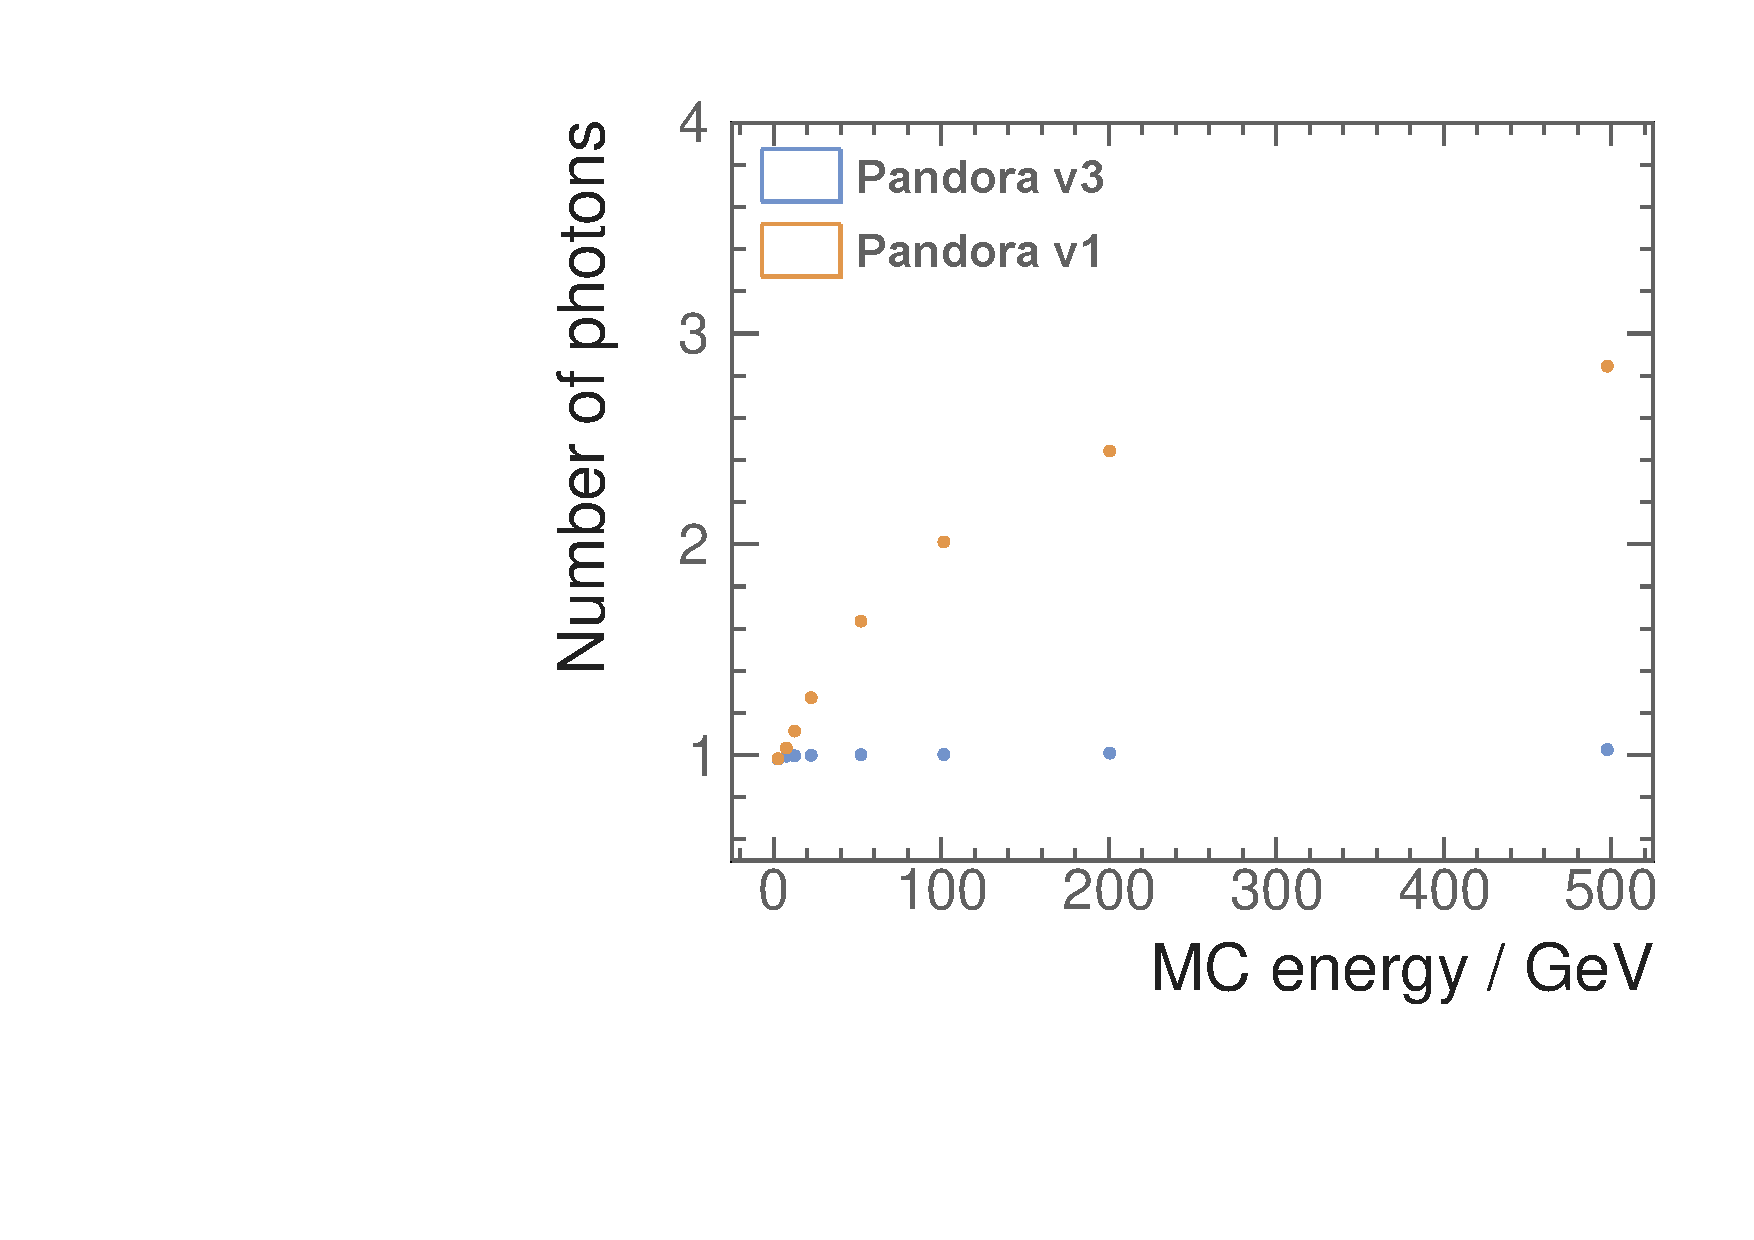
\includegraphics[width=\textwidth]{photon/SingleN_pedit.pdf}
        \caption{}
        \label{fig:photonSingleN_p}
    \end{subfigure}
    \begin{subfigure}[b]{0.45\textwidth}
        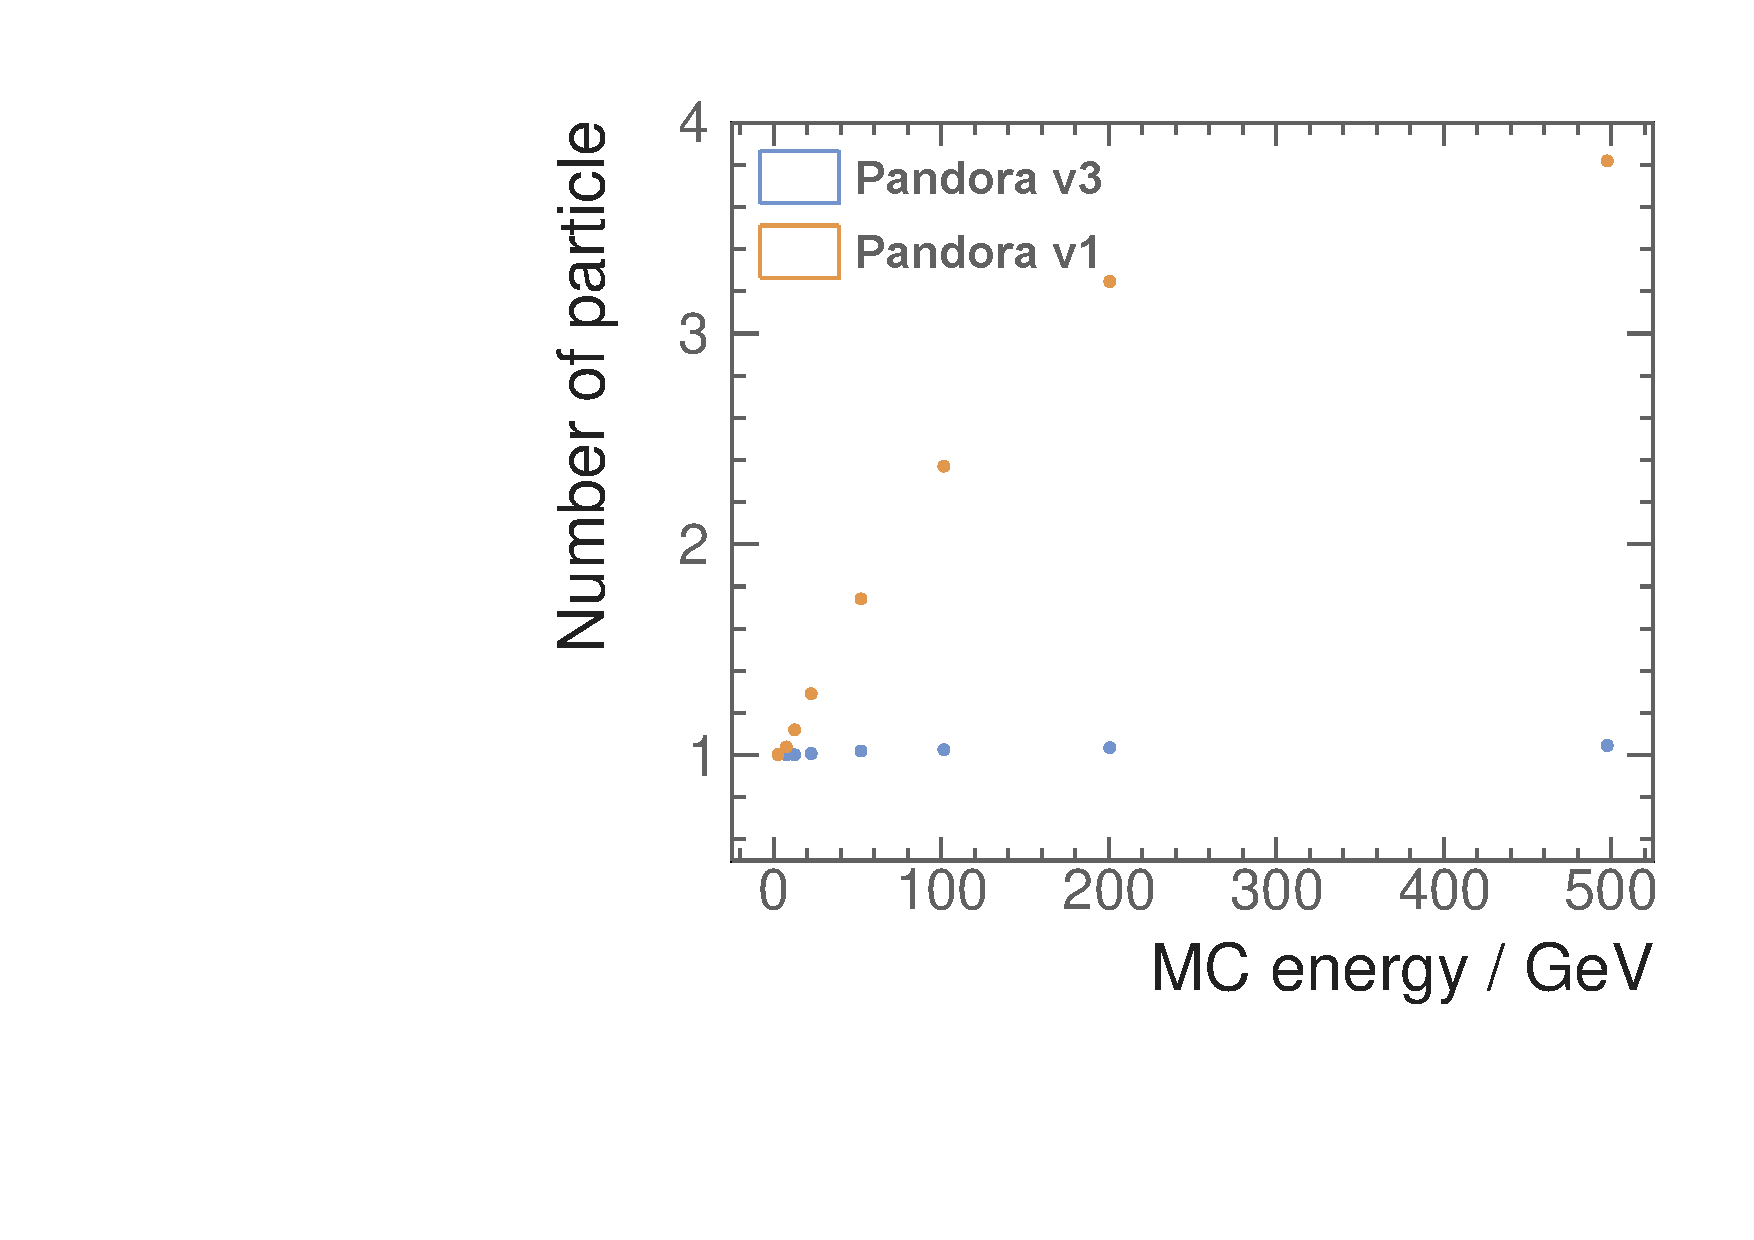
\includegraphics[width=\textwidth]{photon/SingleN_alledit.pdf}
        \caption{}
        \label{fig:photonSingleN_all}
    \end{subfigure}
\caption[]
{\Figure{fig:photonSingleN_p} and \Figure{fig:photonSingleN_all} shows the average number of reconstructed photons and reconstructed particles, as a function of their true energy using a single photon per event sample. The top orange and bottom blue dots are reconstructed with \pandora version 1 and version 3. The photon reconstruction is changed in \pandora version 2.}
\label{fig:photonSingleN}
\end{figure}



\Figure{fig:photonDoubleCompareN} illustrates a similar reduction in the photon fragments and the neutral hadron fragments using two photons of 500 and 50\,GeV per event sample. The high energy photon are more likely to create fragments. And the imbalance in the two photon energies makes it more difficult to separate correctly. The figure shows the MC distance separation from 0 to 30\,mm, which corresponds to approximately 6 \ECAL square cell. In both \Figure{fig:photonDoubleCompareN_p} and \Figure{fig:photonDoubleCompareN_all}, the average numbers of photon and particle are below 2.05 at 30\,mm apart, which is significantly better than reconstruction in \pandora version 1. Two photons start to be resolved at 10\,mm apart, and fully resolved at 20\,mm apart. The resolution is better than reconstruction in \pandora version 1, which is difficult to extract due to excess fragments.


\begin{figure}[tbph]
\centering
    \begin{subfigure}[b]{0.45\textwidth}
        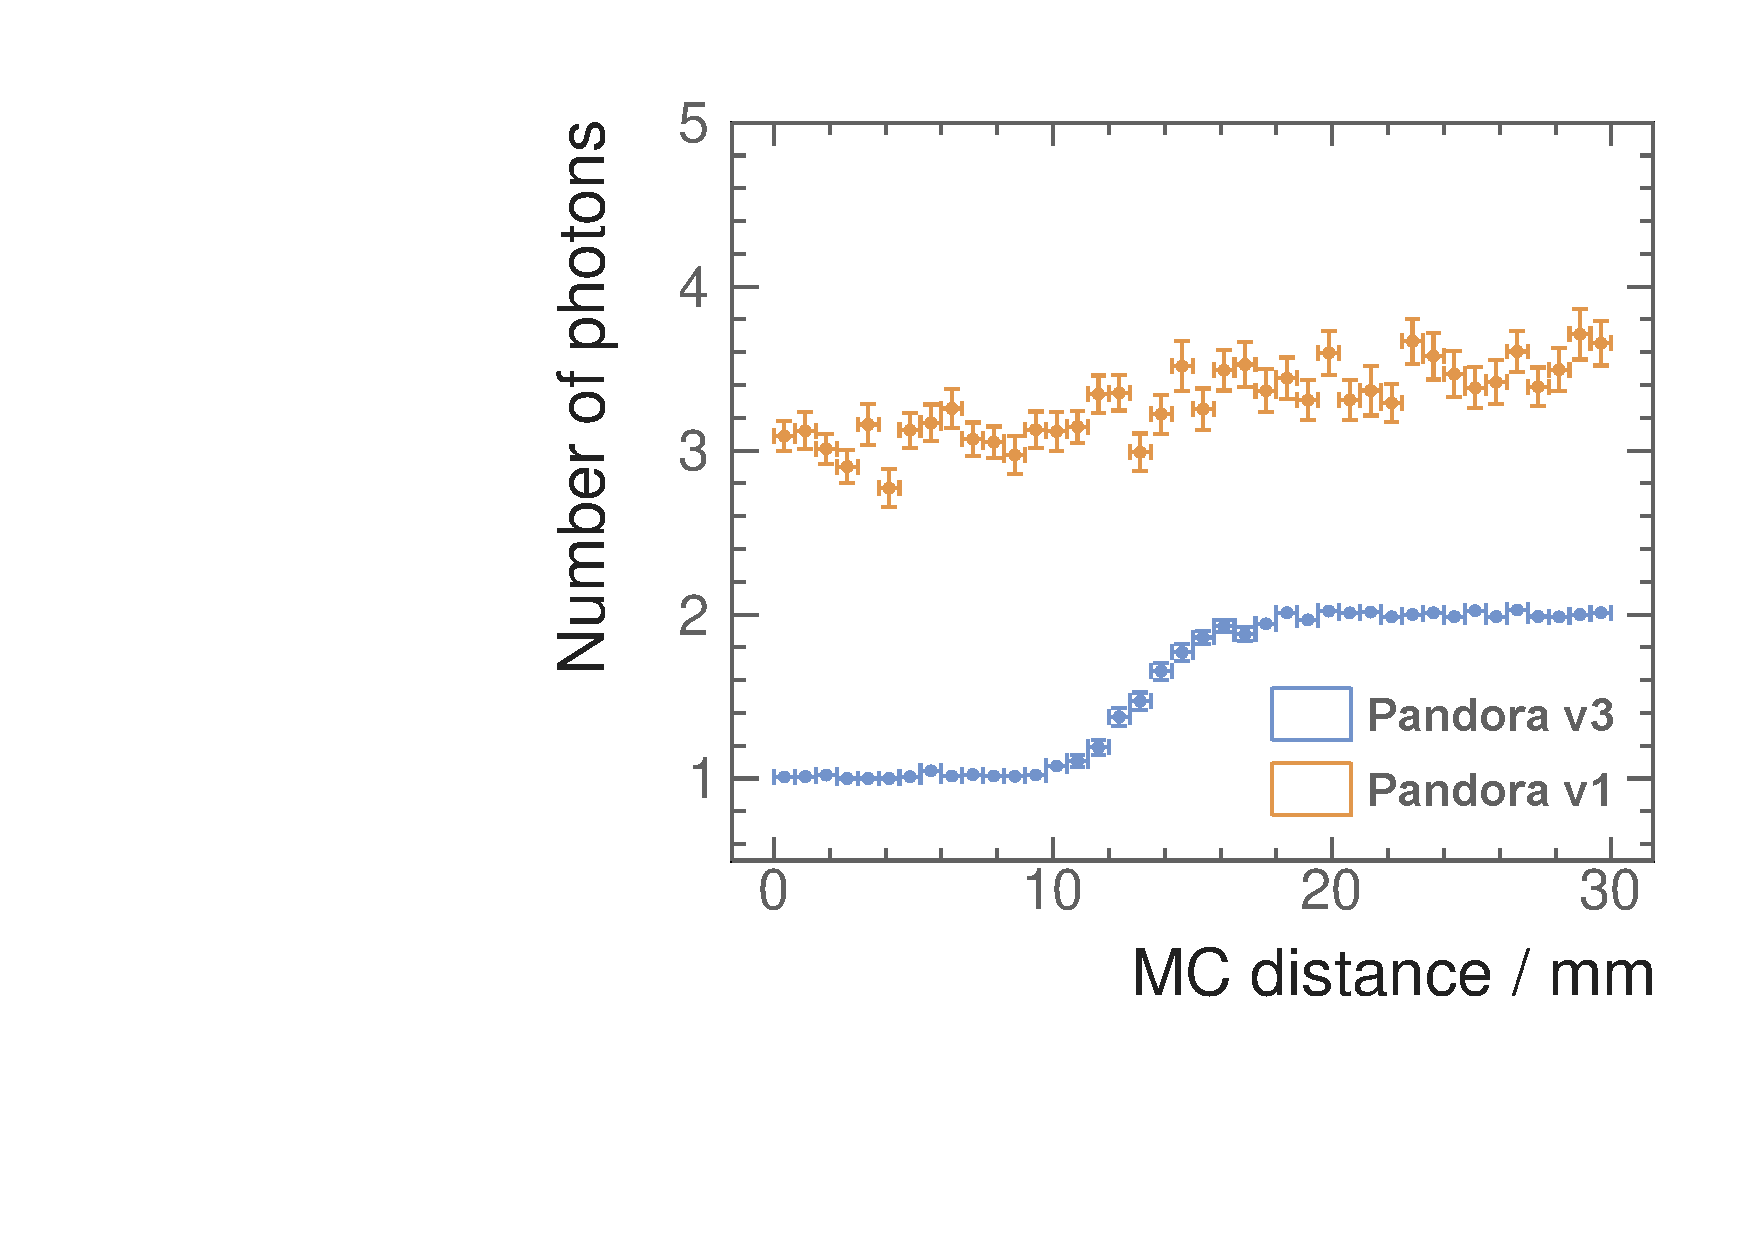
\includegraphics[width=\textwidth]{photon/DoubleCompareN_p3edit.pdf}
        \caption{}
        \label{fig:photonDoubleCompareN_p}
    \end{subfigure}
    \begin{subfigure}[b]{0.45\textwidth}
        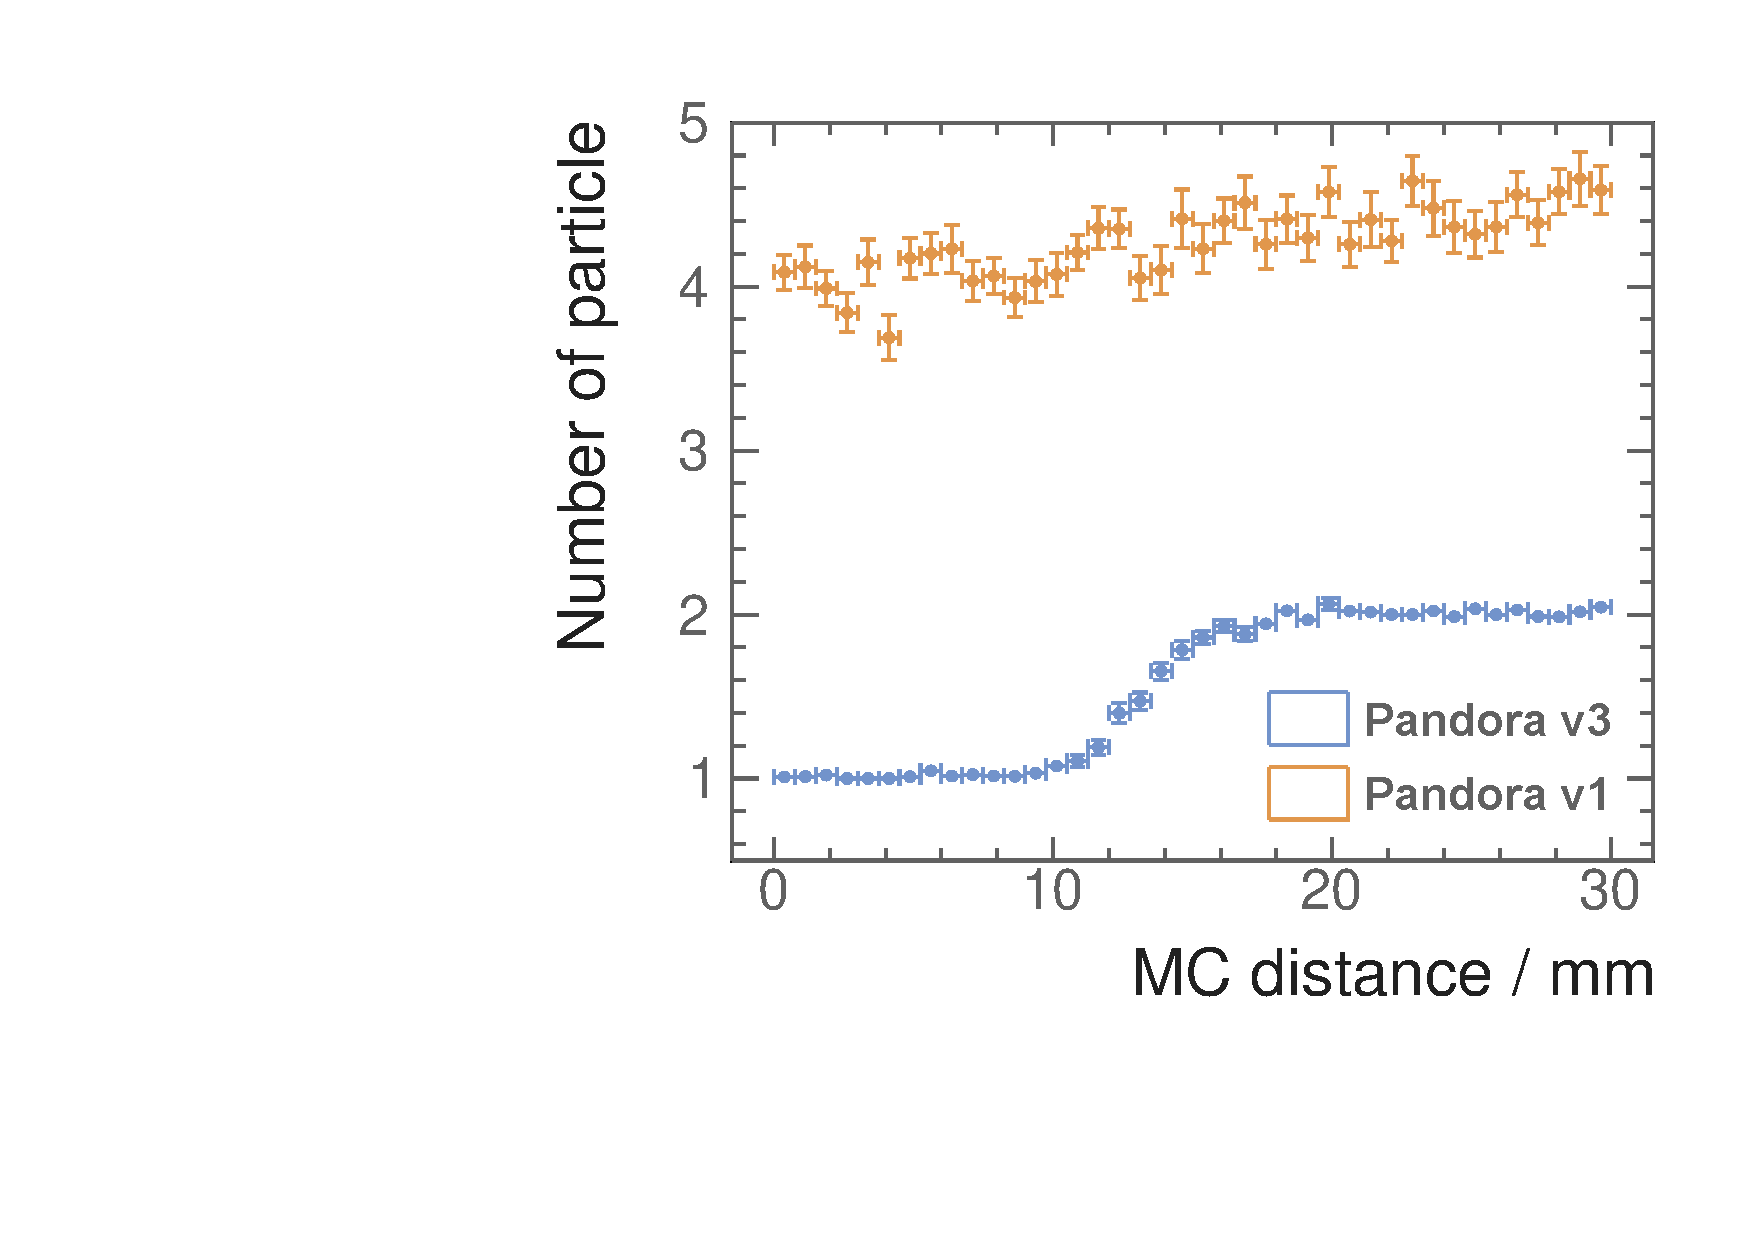
\includegraphics[width=\textwidth]{photon/DoubleCompareN_all2edit.pdf}
        \caption{}
        \label{fig:photonDoubleCompareN_all}
    \end{subfigure}

\caption[]
{\Figure{fig:photonDoubleCompareN_p} and \Figure{fig:photonDoubleCompareN_all} shows the average number of reconstructed photons and reconstructed particles, as a function of the MC distance separation in the calorimeter, using two photons of 500 and 50\,GeV per event sample. The top orange and bottom blue dots are reconstructed with \pandora version 1 and version 3. The photon reconstruction is changed in \pandora version 2.}
\label{fig:photonDoubleCompareN}
\end{figure}

Another metric to reflect the improvement in photon reconstruction is the fragment energy fraction of the total energy as function of the distance separation. Shown in \Figure{fig:photonDoubleFragEnergy}, using two photons of 500 and 50\,GeV per event sample, a reduction in fragment energy can be seen clearly. With improved reconstruction, the average fragment energy fraction is below 0.1\% up to 30\,mm apart, whilst around 5\% energy would be in fragments with reconstruction in \pandora version 1.


\begin{figure}[tbph]
\centering
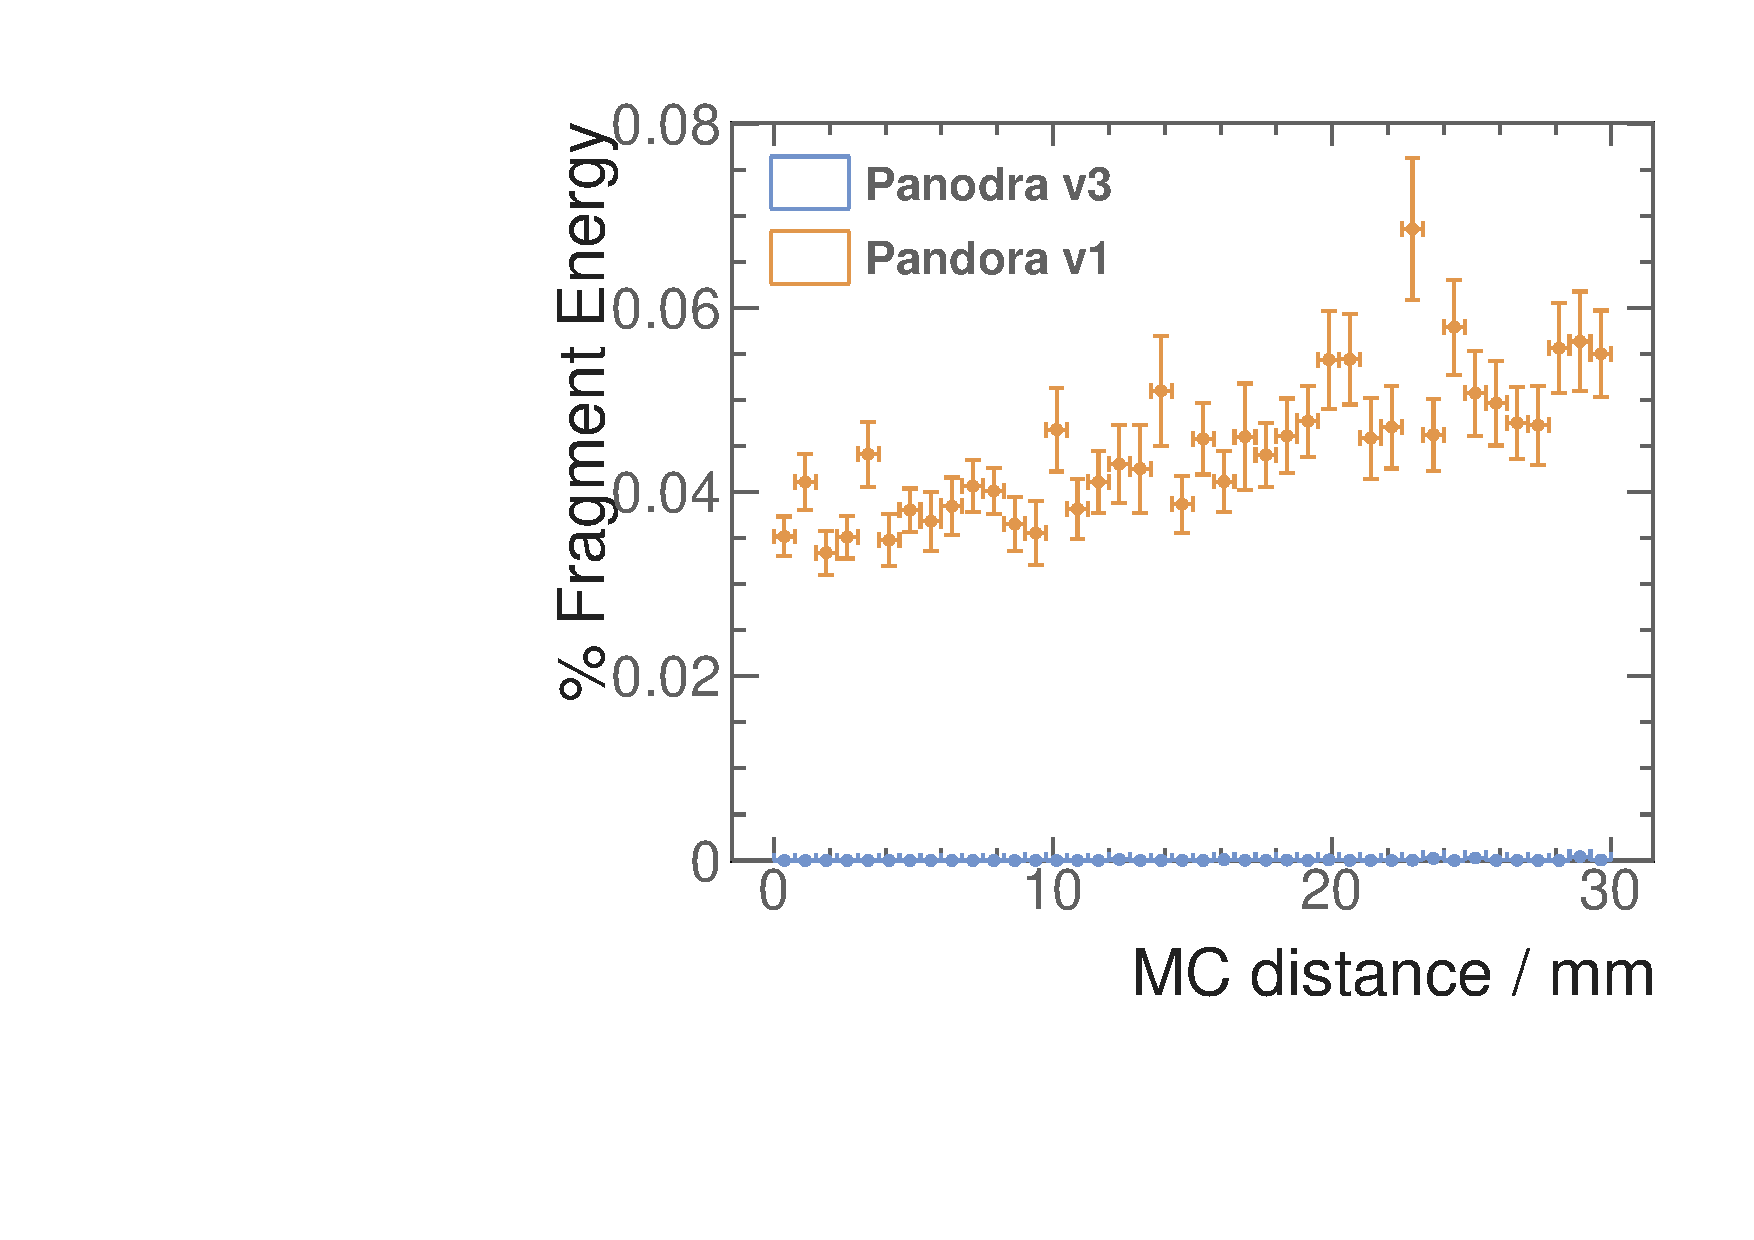
\includegraphics[width=0.45\textwidth]{photon/DoubleCompareFragEnergy.pdf}
\caption[]
{\Figure{fig:photonDoubleFragEnergy} shows the average fraction fragments energies of the total energy, as a function of the MC distance separation in the calorimeter, using two photons of 500 and 50\,GeV per event sample. The top orange and bottom blue dots are reconstructed with \pandora version 1 and version 3. The photon reconstruction is changed in \pandora version 2.}
\label{fig:photonDoubleFragEnergy}
\end{figure}

TODO
write RMS90

The improvement in completeness and resolution in photon reconstruction, as shown in single photon and double photon reconstruction, leads to a small improvement in the jet energy resolution at high energy. Jet energy resolution is defined as the root mean squared divided by the mean for the smallest width of distribution that contains 90\% of entries, using \Zuds sample. The di-jet energy is sampled at 91, 200, 360 and 500\,GeV. Shown in \Figure{fig:photonJER}, the jet energy resolutions are better at 360 and 500\,GeV with improved photon reconstruction.


\begin{figure}[tbph]
\centering
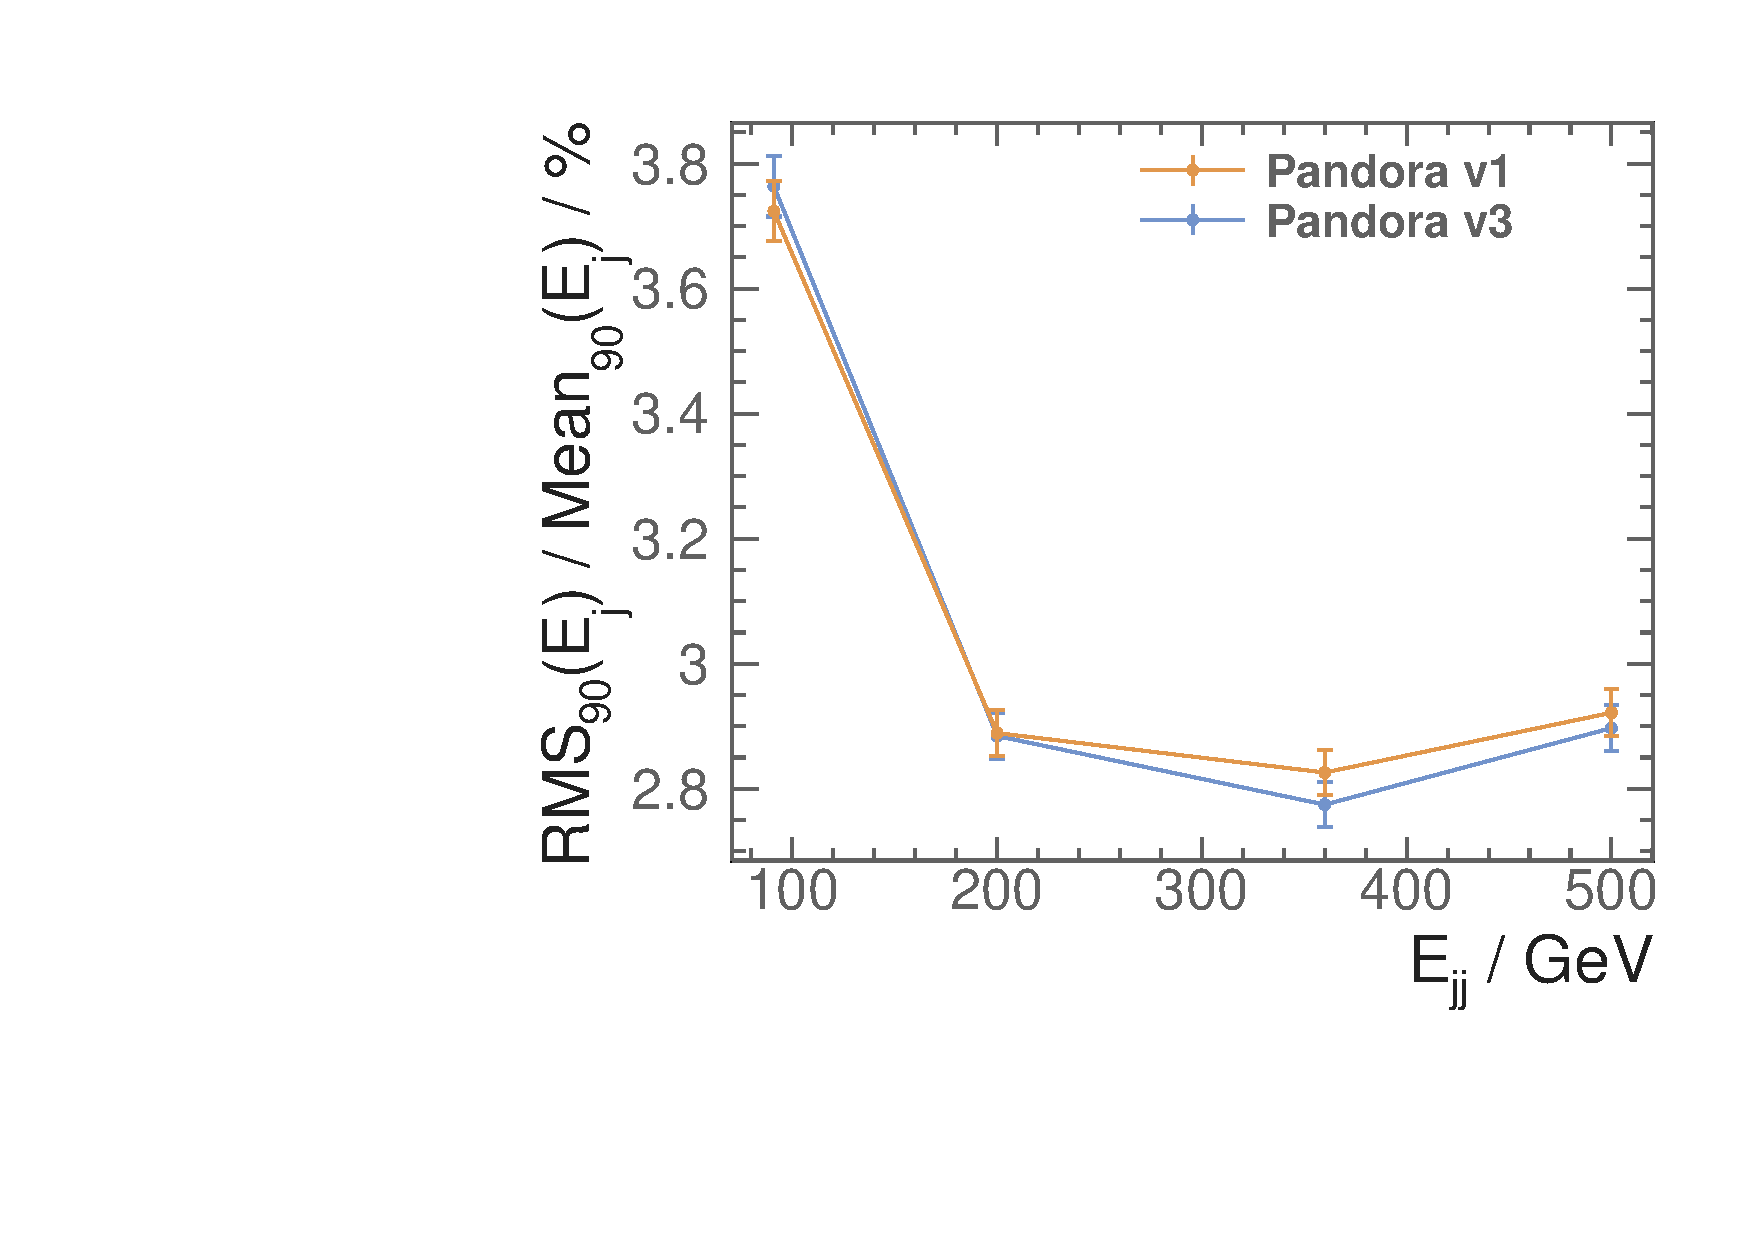
\includegraphics[width=0.45\textwidth]{photon/JERnew.pdf}
\caption[]
{\Figure{fig:photonJER} shows jet energy resolution as a function of the di-jet energy using \Zuds sample. The top orange and bottom blue dots are reconstructed with \pandora version 1 and version 3. The photon reconstruction is changed in \pandora version 2.}
\label{fig:photonJER}
\end{figure}

The improvement of the photon is also demonstrated in \Chapter{chap:Tau}, where tau lepton decay modes are classified. Excellent photon reconstruction leads to a high classification rate.

TODO
write other people using it

\section{Breakdown of photon reconstruction improvement}

As stated before, photon reconstruction algorithm in \Section{sec:photonRecostrcution} and photon splitting algorithm in \Section{sec:photonSplitting}  improves the photon completeness and the photon pair resolution. The fragment removal algorithm in \Section{sec:photonFragRemoval} removes fragments in the \ECAL. High energy fragment removal algorithm in \Section{sec:photonHighEFragRemoval} removes fragments in the \HCAL. To show the incremental improvement, the average number of particle for a high energy photon pair, 500 - 500\,GeV is shown in \Figure{fig:photonDoubleCompareAlgs}. With fragment removal algorithm in the \ECAL, the number of fragment is reduced significantly comparing to \Figure{fig:photonDoubleCompareN_all}, shown as the orange dots. The high energy fragment removal algorithm further reduces the number of fragments, shown as the green dots. At 40\,mm apart, with both fragment removal algorithms, there is less than 0.05 fragment per photon pair, which is similar to the best performance. The introduction of the revised photon reconstruction and photon splitting improves the photon separation resolution. Photons pair starts to be resolved at 5\,mm instead of 10\,mm for 500 - 500\,GeV pair. Also two photons are fully resolved at 15\,mm instead of 40\,mm apart.

\begin{figure}[tbph]
\centering
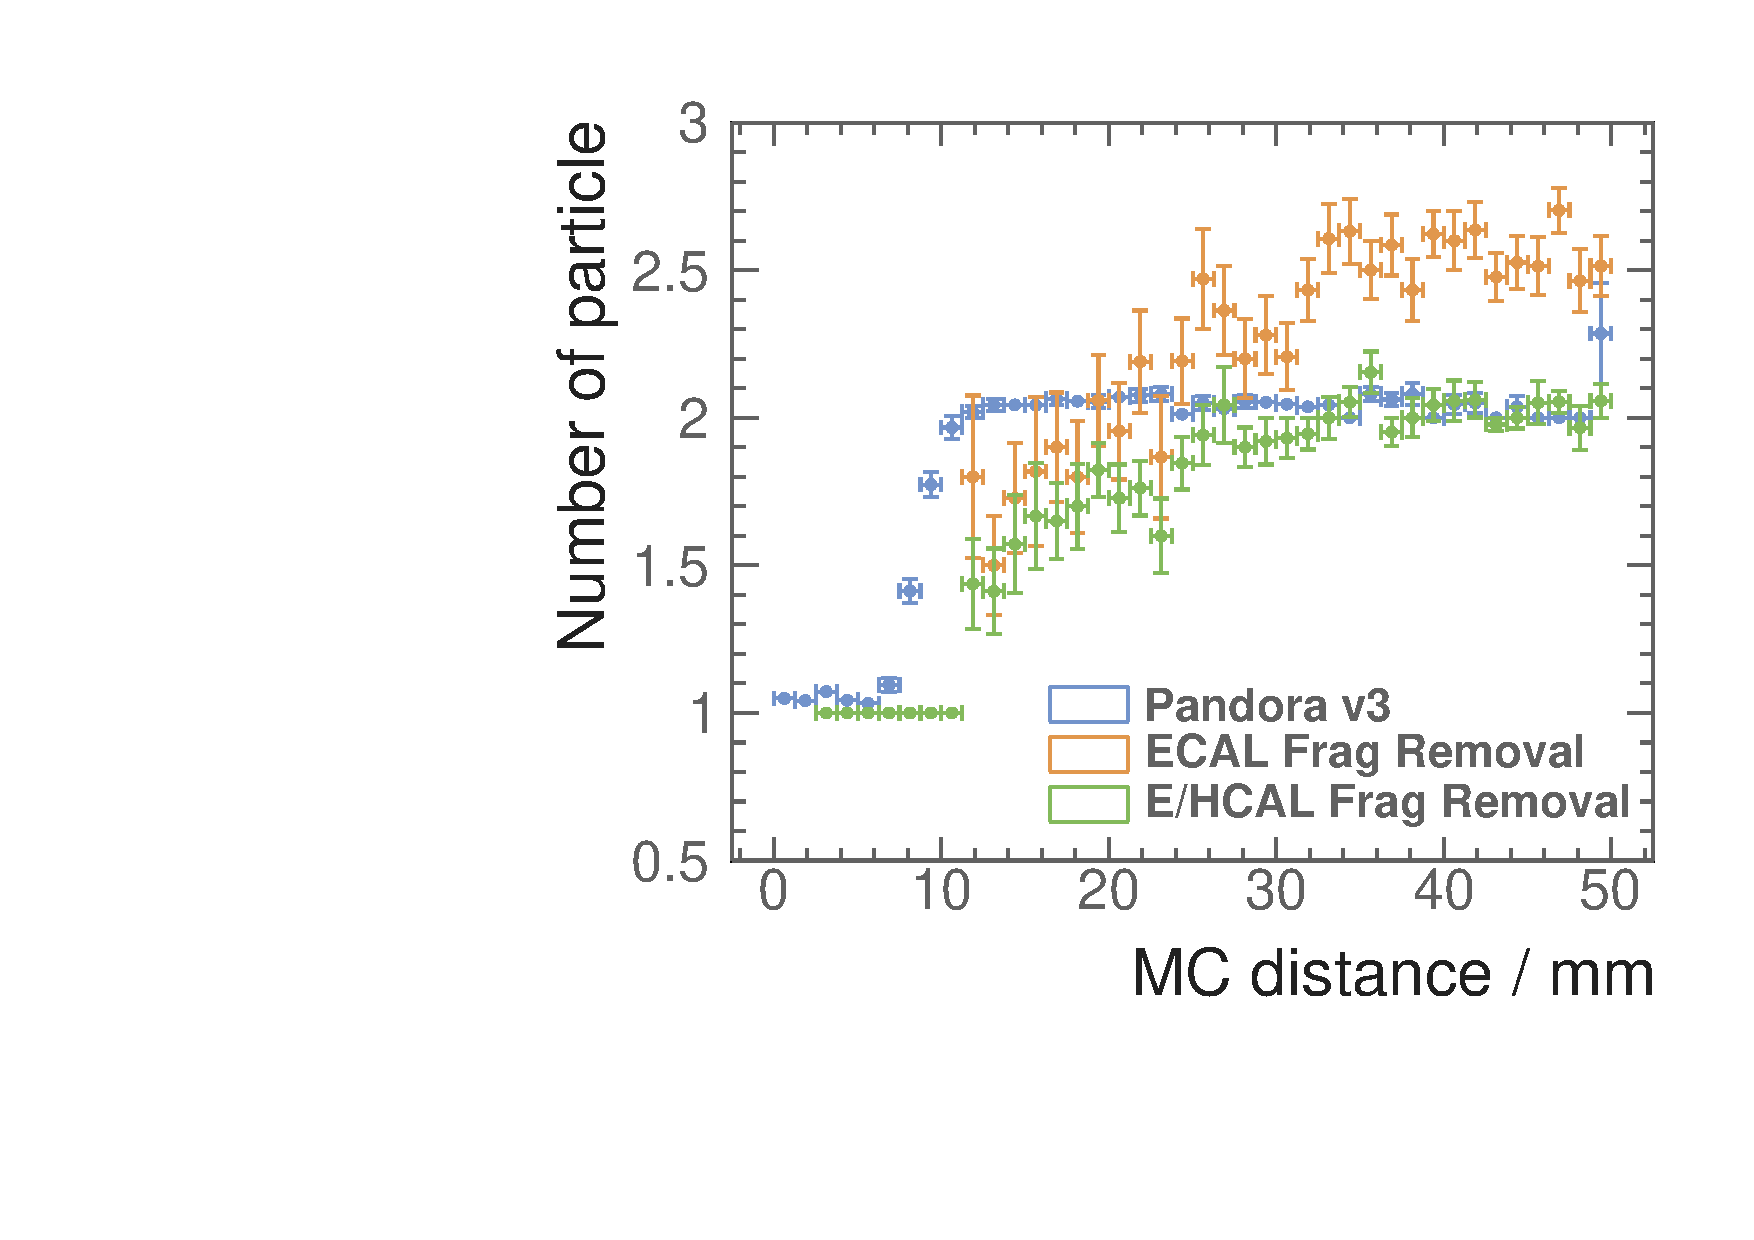
\includegraphics[width=0.45\textwidth]{photon/DoubleCompareAlgs.pdf}
\caption[]
{Figure shows the average number of photons, as a function of the MC distance separation in the calorimeter, using two photons of 500 and 500\,GeV per event sample. The blue, orange, and green dots are reconstructed with \pandora version 3, \pandora version 1 with fragment removal in the \ECAL (\Section{{sec:photonFragRemoval}}), and \pandora version 1 with fragment removal in the \ECAL and the \HCAL. The photon reconstruction is changed in \pandora version 2.}
\label{fig:photonDoubleCompareAlgs}
\end{figure}

\section{Photon reconstruction performance}

In \Section{sec:photonPerformanceCompare}, the improved performance of the photon reconstruction is demonstrated with different metrics, using single photon, double photons and jet samples. In this section, the features of the photon reconstruction will be described.

For simple samples such as two photons per event, there are very few fragments. Shown in \Figure{fig:photonDoubleCompareN_pN_all} for 500 and 50\,GeV photons pair sample, the average number of photons beyond 20\,mm apart is 2 within errors. The average number of particle is less than 0.05 larger than the average number of photons.

\begin{figure}[tbph]
\centering
    \begin{subfigure}[b]{0.45\textwidth}
        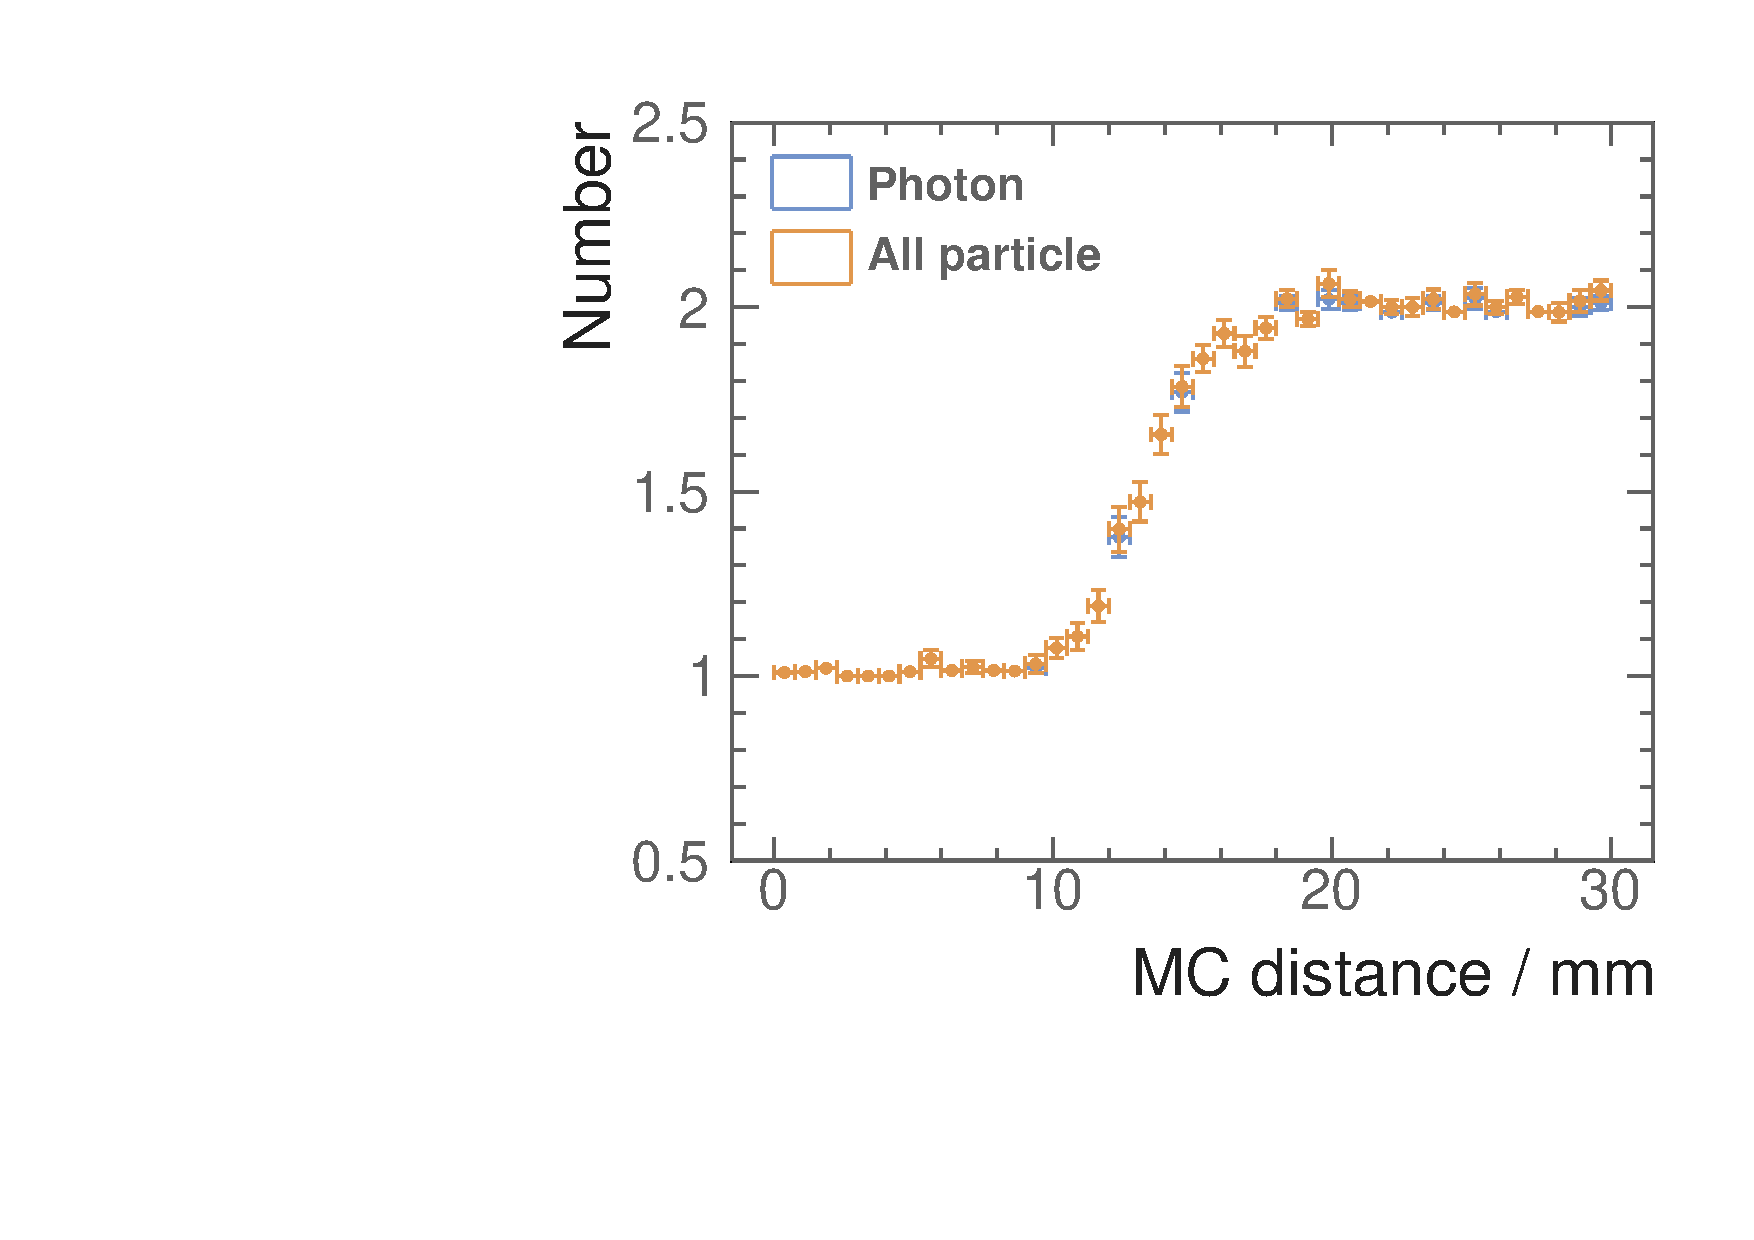
\includegraphics[width=\textwidth]{photon/DoubleN_pN_all.pdf}
        \caption{}
        \label{fig:photonDoubleCompareN_pN_all}
    \end{subfigure}
    \begin{subfigure}[b]{0.45\textwidth}
        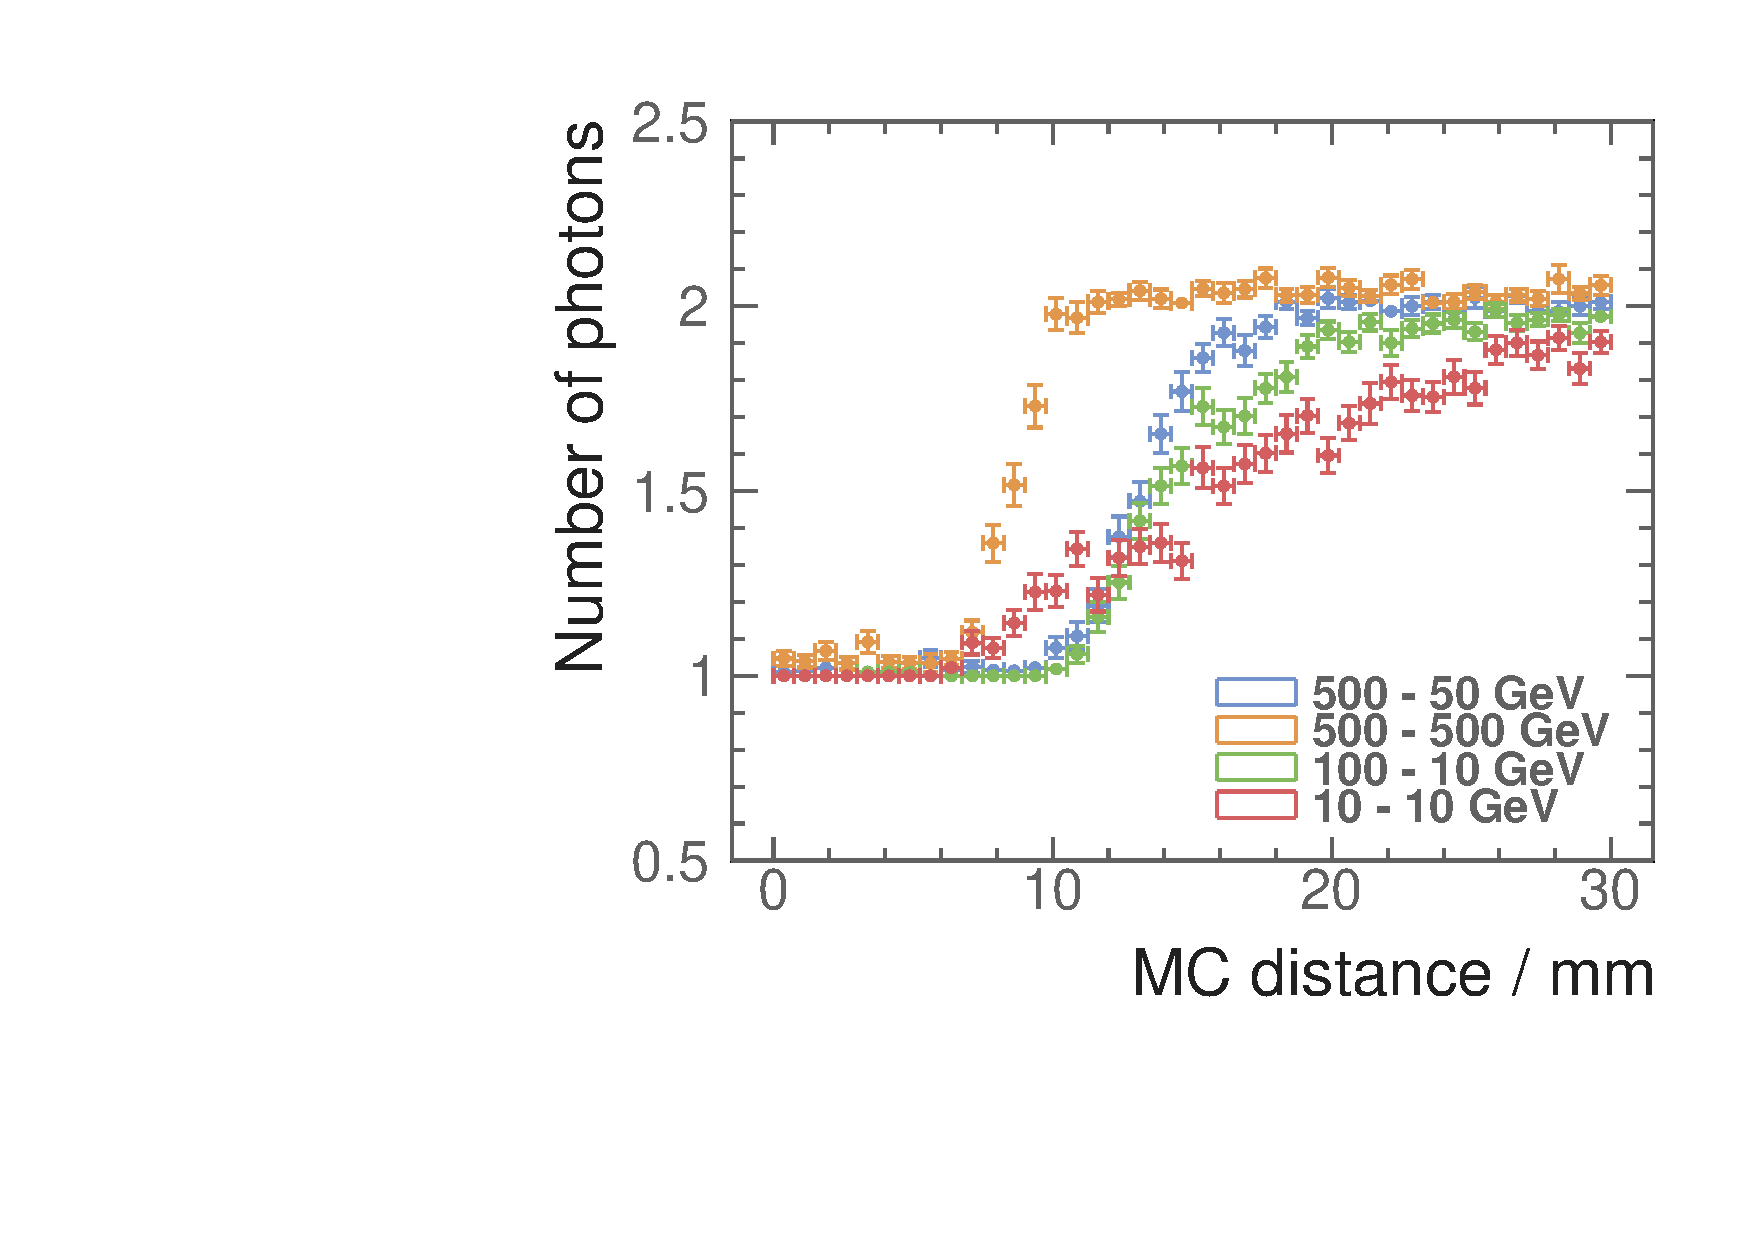
\includegraphics[width=\textwidth]{photon/DoubleCompareEnergies.pdf}
        \caption{}
        \label{fig:photonDoubleCompareEnergies}
    \end{subfigure}
\caption[]
{\Figure{fig:photonDoubleCompareN_pN_all} shows the average numbers of photon and particle using two photons of 500 and 50\,GeV per event sample. \Figure{fig:photonDoubleCompareEnergies} shows the  average numbers of photon for four different photon pairs: 500 - 50, 500 - 500, 100 - 10 and 10 - 10\,GeV.}
\label{fig:photonDoublePerformance}
\end{figure}

The resolving power of a photon pair depends on energies of two photons. \Figure{fig:photonDoubleCompareEnergies} is an example of average number of photon reconstructed for differen photon pairs. When the energies of two photons are similar, the resolving distance is shorter. This is because that the two photon showers have similar sizes, and the peak finding algorithm can exploit the symmetry. For example, 500 - 500\,GeV photon pair and 10 - 10\,GeV photon pair start to be resolved at 6\,mm apart, which is about 1 \ECAL cell. The asymmetrical photon pair,  500 - 50\,GeV and  100 - 10\,GeV pair, starts to be resolved at 10\,mm apart, which is about 2 \ECAL cell.

For the energetic photon, it is more difficult to remove fragments, but it is easier to identify the photon. The electromagnetic shower core is more dominant than the peripherals. Therefore separating two energetic photons is easier than separating two low energy photons. This can be seen in \Figure{fig:photonDoubleCompareEnergies}. At 20\,mm apart, two photons in  500 - 500\,GeV pair are fully resolved, where approximately 60\% of two photons in 10 - 10\,GeV pair are resolved.

